%% Author:      Chris Coulston
%% Purp:        Here are the homework problems and their solutions.

%%\documentclass[11pt,psfig]{book}
\documentclass[letterpaper, 10pt]{memoir}
\chapterstyle{ger}
\settrims{0pt}{0pt}
\semiisopage[9]		% [N] is spine margin is 1/Nth pf page 


% To keep the book.tex file clean, I pulled all the formating and package 
% includes into the preamble.tex file
%%------------------------------------------------------
%%------------------------------------------------------

\usepackage{amsmath,amssymb}
\usepackage{lmodern}
\usepackage{iftex}

\usepackage{xcolor}
\usepackage{graphicx}

\usepackage{dirtree}		% For the body of knowledge


\usepackage{listings}

\makeatletter
\def\maxwidth{\ifdim\Gin@nat@width>\linewidth\linewidth\else\Gin@nat@width\fi}
\def\maxheight{\ifdim\Gin@nat@height>\textheight\textheight\else\Gin@nat@height\fi}
\makeatother
% Scale images if necessary, so that they will not overflow the page
% margins by default, and it is still possible to overwrite the defaults
% using explicit options in \includegraphics[width, height, ...]{}
\setkeys{Gin}{width=\maxwidth,height=\maxheight,keepaspectratio}
% Set default figure placement to htbp
\makeatletter
\def\fps@figure{htbp}
\makeatother

\usepackage{longtable,booktabs,array}
\usepackage{multirow}
\usepackage{calc}
\usepackage[normalem]{ulem}

\usepackage{pdflscape}

\usepackage{bookmark}

\usepackage{xurl}

\usepackage{hyperref}

%\let\oldhypertarget\hypertarget
%\renewcommand*{\hypertarget}{\oldhypertarget\space}



\hypersetup{
   colorlinks=true,
   linkcolor=red}

\makeindex

\begin{document}

\frontmatter
 \title{}
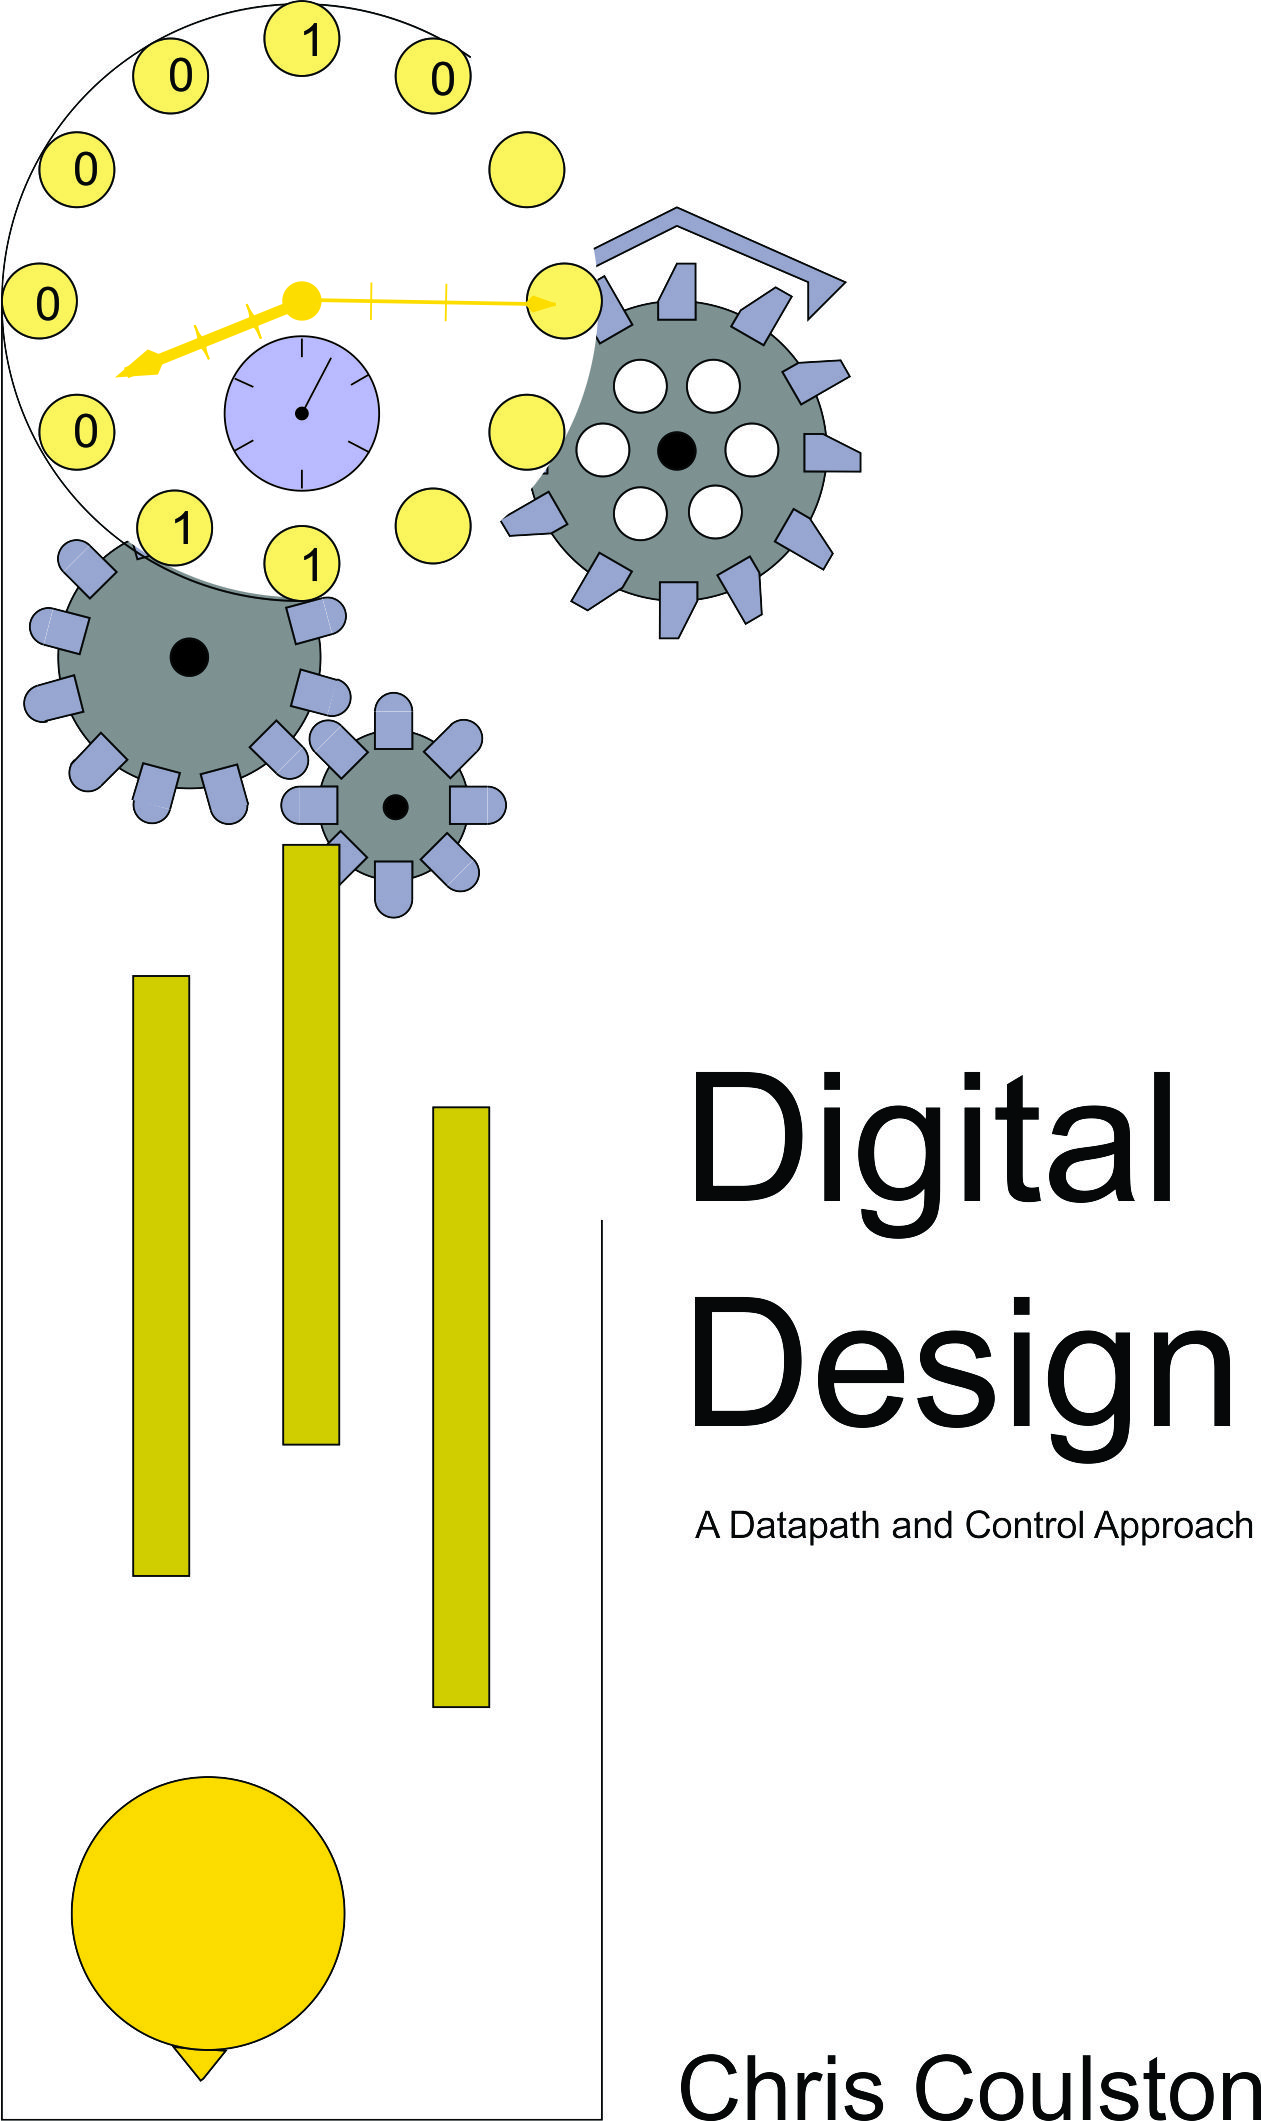
\includegraphics{./Fig/colorCover}
 \maketitle
 
 
This document was prepared with \LaTeX.
\vspace{2cm}

Digital Design - A Datapath and Control Approach © 2024 by Christopher Coulston is licensed under CC BY-NC-SA 4.0
For more infomation about the Create Commons license see: https://creativecommons.org/licenses/by-nc-sa/4.0/

\begin{figure}[h]
    
\includegraphics[width=1cm]{./Fig/cc-logo.pdf}
    
\includegraphics[width=1cm]{./Fig/cc-by.pdf}
    
\includegraphics[width=1cm]{./Fig/cc-nc.pdf}
    
\includegraphics[width=1cm]{./Fig/cc-sa.pdf}
\end{figure}

\tableofcontents
\showanswers

\mainmatter

\chapter{Numbering Systems}
\section{Exercises}
\label{section:chap01Exercises}

\begin{enumerate}
\item \textbf{ (1 pt. each)} Syllabus:
	\begin{enumerate}
	\item What is the late penalty for homework?
	
	\begin{onlysolution}
	\itshape
	There is a 33\% deduction per day.
	\end{onlysolution}

	\item True or False: Calculators can be used during exams.
	
	\begin{onlysolution}
	\itshape
	You cannot use calculators at my exams.
	\end{onlysolution}
	
	
	\item True of False: University ID is required during exams.
	
		
	\begin{onlysolution}
	\itshape
	I check ID at the exams.  After I learn 
		your names its not such a big
		deal, but bring it to be safe.
	\end{onlysolution}
	
	\item What is my thesis regarding grades?
	\item Bob L. Student has the following grades.  Determine his final
	overall course percentage and grade.

		\begin{tabular}{l|l}
		Component & Percentage \\ \hline \hline
		Homework & $60\%$ \\ \hline
		Exam 1	 & $90\%$ \\ \hline
		Exam 2	 & $80\%$ \\ \hline
		Final	 & $70\%$ \\ 
		\end{tabular}


	\begin{onlysolution}
	\itshape
                \begin{tabular}{l|l|l}
                Component & Percentage & Weight \\ \hline \hline
                Homework & $60\%$    & 60*0.35 = 21\\ \hline
                Exam 1   & $90\%$    & 90*0.20 = 18\\ \hline
                Exam 2   & $80\%$    & 80*0.20 = 16\\ \hline
                Final    & $70\%$    & 70*0.25 = 17.5 \\ \hline
                Total    & $72.5\%$ & C \\
                \end{tabular}
	\end{onlysolution}

	\item How should you prepare for the 43$^{rd}$ lecture?

	\begin{onlysolution}
	\itshape
	 Look over homework problem 8.10, page 165
	 \end{onlysolution}
	 
	\end{enumerate}

\item \textbf{ (1 pt. each)} Convert the following numbers to decimal. 
Show work, or receive 1/2 credit.
	\begin{enumerate}
	\item $100_2$
	\begin{onlysolution}	\itshape $100_2 = 2^2 = 4_{10}$\end{onlysolution}
	
	\item $1000_2$
	\begin{onlysolution}	\itshape $1000_2 = 2^3 = 8_{10}$\end{onlysolution}
	
	\item $10000_2$
	\begin{onlysolution}	\itshape $10000_2 = 2^4 = 16_{10}$\end{onlysolution}
	
	\item $100000_2$
	\begin{onlysolution}	\itshape $100000_2 = 2^5 = 32_{10}$\end{onlysolution}
	
	\item $111111_2$
	\begin{onlysolution}	\itshape $111111_2 = 2^5+2^4+2^3+2^2+2^1+2^0=63_{10}$\end{onlysolution}
	
	\item $1000100101000101_2$
	\begin{onlysolution}	\itshape $1000100101000101_2=2^{15}+2^{11}+2^8+2^6+2^5+2^0=35141_{10}$\end{onlysolution}
	
	\item $3EA_{16}$
	\begin{onlysolution}	\itshape$3EA_{16}=0011 1110 1010 = 2^9+2^8+2^7+2^6+2^5+2^3+2^1=1002_{10}$\end{onlysolution}
	
     \end{enumerate}


\item \textbf{ (1 pt. each)} Convert the following number to binary. Show 
work, or receive 1/2 credit.
	\begin{enumerate}
	\item $44_{16}$
	\begin{onlysolution}	\itshape $44_{16} =0100 0100_2$\end{onlysolution}
	
	\item $44_{10}$
	\begin{onlysolution}	\itshape $44_{10} = 32+8 = 2^5+2^3=101100_2$\end{onlysolution}
	
	\item $1023_{10}$
	\begin{onlysolution}	\itshape$1023_{10} = 512+256+128+64+32+16+8+4+2+1=
        2^9+2^8+2^7+2^6+2^5+2^4+2^3+2^2+2^1+2^0=1111111111_2$\end{onlysolution}
        
	\end{enumerate}


\item \textbf{ (1 pt. each)} Convert the following number to hex. Show work, or receive 1/2 credit.
	\begin{enumerate}
	
	\item $101011101_2$
	\begin{onlysolution}	\itshape$1 0101 1101_2 = 15D_{16}$ \end{onlysolution}
	
	\item $77_{10}$
	\begin{onlysolution}	\itshape $77_{10} = 64+8+4+1=2^6+2^3+2^2+2^0=100 1101_2=4D_{16}$ \end{onlysolution}
	
	\end{enumerate}


\item \textbf{ (2 pts. each)} Toughies:
	\begin{enumerate}
	\item Convert $123_5$ to base-12
	\begin{onlysolution} 	\itshape
		$123_5 = 1*5^2 + 2*5^1 + 3*5^0 = 25+10+3=38_{10}=
        3*12^1 + 2*12^0 = 32_{12}$ \end{onlysolution}
        
	\item Convert $789_{12}$ to base-5
	\begin{onlysolution}
	\itshape	$789_{12} = 7*12^2+8*12^1+9*12^0=1008+96+9=1113_{10}= \\
        1*5^4+3*5^3 + 4*5^2 + 2*5^1 + 3*5^0 = 13423_5$ \end{onlysolution}
        
	\item What is the largest base-10 quantity that can be represented
	using 5 digits in base 12?

	\begin{onlysolution}
	\itshape $BBBBB_{12} = 11*12^4+11*12^3+11*12^2+11*12^1+11*12^0=248831_{10}$ \end{onlysolution}
	
	\end{enumerate}


\item \textbf{ (1 pt. each)} Perform the following additions, assume a word 
size of four bits. Determine if overflow occurs.
	\begin{enumerate}
	
	\item $0110_2 + 0101_2$
	\begin{onlysolution}	\itshape0110 + 0101 = 1011\end{onlysolution}
	
	\item $0010_2 + 0110_2$
	\begin{onlysolution}	\itshape0010 + 0110 = 1000\end{onlysolution}
	
	\item $0111_2 + 0011_2$
	\begin{onlysolution}	\itshape0111 + 0011 = 1010\end{onlysolution}
	
	\item $0010_2 + 0101_2$
	\begin{onlysolution}	\itshape0010 + 0101 = 0111\end{onlysolution}
	
	\item $0010_2 + 1010_2$
	\begin{onlysolution}	\itshape0010 + 1010 = 1100\end{onlysolution}
	
	\item $0101_2 + 1011_2$
	\begin{onlysolution}	\itshape0101 + 1011 = 10000 overflow\end{onlysolution}
	
	\item $0011_2 + 1001_2$
	\begin{onlysolution}	\itshape0011 + 1001 = 1100\end{onlysolution}
	
	\end{enumerate}
\end{enumerate}


\chapter{Representations of Logical Functions}
\begin{enumerate}
\item {\bf(2 pts. each)} Given: $F(A,B,C,D) = (AB' + (C+(AD)')(BD))'$
\begin{enumerate}
	\item Determine the truth table for $F(A,B,C,D)$

\begin{solution}{ 
Let T3 = C+(AD)'\\
T4 = BD\\
T1 = AB'
T5 = T3 * T4\\

\begin{tabular}{l|l|l|l|l|l|l|l|l|l|l} 
 A &  B &  C &  D & AB' & (AD)' & C+(AD)' & BD & T3*T4 & T1+T5  &  F \\ \hline
 0 &  0 &  0 &  0 &  0  &  1    &  1      &  0 & 0     &  0     &  1  \\ \hline
 0 &  0 &  0 &  1 &  0 &  1 &  1 &  0 & 0 &  0 &  1  \\ \hline
 0 &  0 &  1 &  0 &  0 &  1 &  1 &  0 & 0 &  0 &  1  \\ \hline
 0 &  0 &  1 &  1 &  0 &  1 &  1 &  0 & 0 &  0 &  1  \\ \hline
 0 &  1 &  0 &  0 &  0 &  1 &  1 &  0 & 0 &  0 &  1  \\ \hline
 0 &  1 &  0 &  1 &  0 &  1 &  1 &  1 & 1 &  1 &  0  \\ \hline
 0 &  1 &  1 &  0 &  0 &  1 &  1 &  0 & 0 &  0 &  1  \\ \hline
 0 &  1 &  1 &  1 &  0 &  1 &  1 &  1 & 1 &  1 &  0  \\ \hline
 1 &  0 &  0 &  0 &  1 &  1 &  1 &  0 & 0 &  1 &  0  \\ \hline
 1 &  0 &  0 &  1 &  1 &  0 &  0 &  0 & 0 &  1 &  0  \\ \hline
 1 &  0 &  1 &  0 &  1 &  1 &  1 &  0 & 0 &  1 &  0  \\ \hline
 1 &  0 &  1 &  1 &  1 &  0 &  1 &  0 & 0 &  1 &  0  \\ \hline
 1 &  1 &  0 &  0 &  0 &  1 &  1 &  0 & 0 &  0 &  1  \\ \hline
 1 &  1 &  0 &  1 &  0 &  0 &  0 &  1 & 0 &  0 &  1  \\ \hline
 1 &  1 &  1 &  0 &  0 &  1 &  1 &  0 & 0 &  0 &  1  \\ \hline
 1 &  1 &  1 &  1 &  0 &  0 &  1 &  1 & 1 &  1 &  0  \\  
\end{tabular} 
} \end{solution}

	\item Draw a schematic of the logic circuit which realizes $F$ as
	shown, i.e. do not use Boolean Algebra on $F$.

\begin{solution}{
	\begin{figure}[ht]
	\center{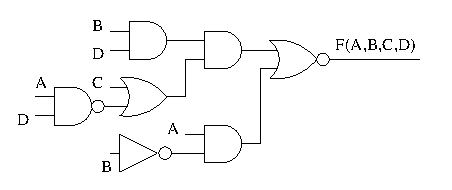
\includegraphics{./FigHw2/Sol2-1}}
	\end{figure}
}\end{solution}
\end{enumerate}


\item {\bf(2 pts. each)} For the circuit in Figure~\ref{fig:hw2}: 
\begin{enumerate}
	\item Write a Boolean expression for the function.

	\begin{solution}{ F(A,B,C,D) = (AB+C)D'+ABD'}\end{solution}
\item Draw the truth table for the function.


	\begin{solution}{
	\begin{tabular}{l|l|l|l|l|l|l|l}
	 A &  B &  C &  D & AB+C  & (AB+C)D' & ABD'  &  F  \\ \hline
	 0 &  0 &  0 &  0 &  0 &  0 &  0 &  0  \\ \hline
	 0 &  0 &  0 &  1 &  0 &  0 &  0 &  0  \\ \hline
	 0 &  0 &  1 &  0 &  1 &  0 &  0 &  1  \\ \hline
	 0 &  0 &  1 &  1 &  1 &  1 &  0 &  0  \\ \hline
	 0 &  1 &  0 &  0 &  0 &  0 &  0 &  0  \\ \hline
	 0 &  1 &  0 &  1 &  0 &  0 &  0 &  0  \\ \hline
	 0 &  1 &  1 &  0 &  1 &  0 &  0 &  1  \\ \hline
	 0 &  1 &  1 &  1 &  1 &  1 &  0 &  0  \\ \hline
	 1 &  0 &  0 &  0 &  0 &  0 &  0 &  0  \\ \hline
	 1 &  0 &  0 &  1 &  0 &  0 &  0 &  0  \\ \hline
	 1 &  0 &  1 &  0 &  1 &  0 &  0 &  1  \\ \hline
	 1 &  0 &  1 &  1 &  1 &  1 &  0 &  0  \\ \hline
	 1 &  1 &  0 &  0 &  1 &  0 &  1 &  1  \\ \hline
	 1 &  1 &  0 &  1 &  1 &  1 &  0 &  0  \\ \hline
	 1 &  1 &  1 &  0 &  1 &  0 &  1 &  1  \\ \hline
	 1 &  1 &  1 &  1 &  1 &  0 &  0 &  0  \\ 
	\end{tabular}
}\end{solution}
\end{enumerate}
\begin{figure}[ht]
\center{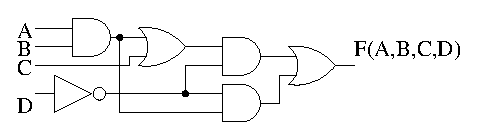
\includegraphics{./FigHw2/Prob2-3}}
\caption{The circuit for Problems 2 and 3.}
\label{fig:hw2}
\end{figure}

\item {\bf(2 pts.)} For the circuit in Figure~\ref{fig:hw2}, show what 
happens when the input (A,B,C,D)=0010 is switched to (A,B,C,D)=1101.
Assume the first input (0010) has been held steady
for a long time.  Use a timing diagram and assume that 
the propagation delay of each gate is 2nS.

	\begin{solution}{ Skipped, a glitch is created for sure.}\end{solution}

\item {\bf (2 pts. each)} For the functions F,G,H,I defined by the 
truth table shown below:
\begin{enumerate}
	\item Determine the canonical SOP and POS realization for $F,G,H,I$.

	\begin{solution}{
F(A,B,C) = (A+B+C)(A+B'+C')(A'+B+C')(A'+B'+C)  =
A'B'C + A'BC' + AB'C' + ABC \\

G(A,B,C) = (A'+B+C)(A'+B'+C') = \\
A'B'C' + A'B'C + A'BC' + A'BC + AB'C + ABC'  \\

H(A,B,C) = (A+B'+C)(A+B'+C')(A'+B+C)(A'+B+C')(A'+B'+C') =\\
A'B'C' + A'B'C + ABC' \\

I(A,B,C) = (A+B+C)(A+B'+C)(A'+B+C)(A'+B'+C) =\\
A'B'C + A'BC + AB'C + ABC \\
}\end{solution}

	\item Draw the circuit diagram for the canonical SOP and POS 
		realization.

	\begin{solution}{
	\begin{figure}[ht]
	\center{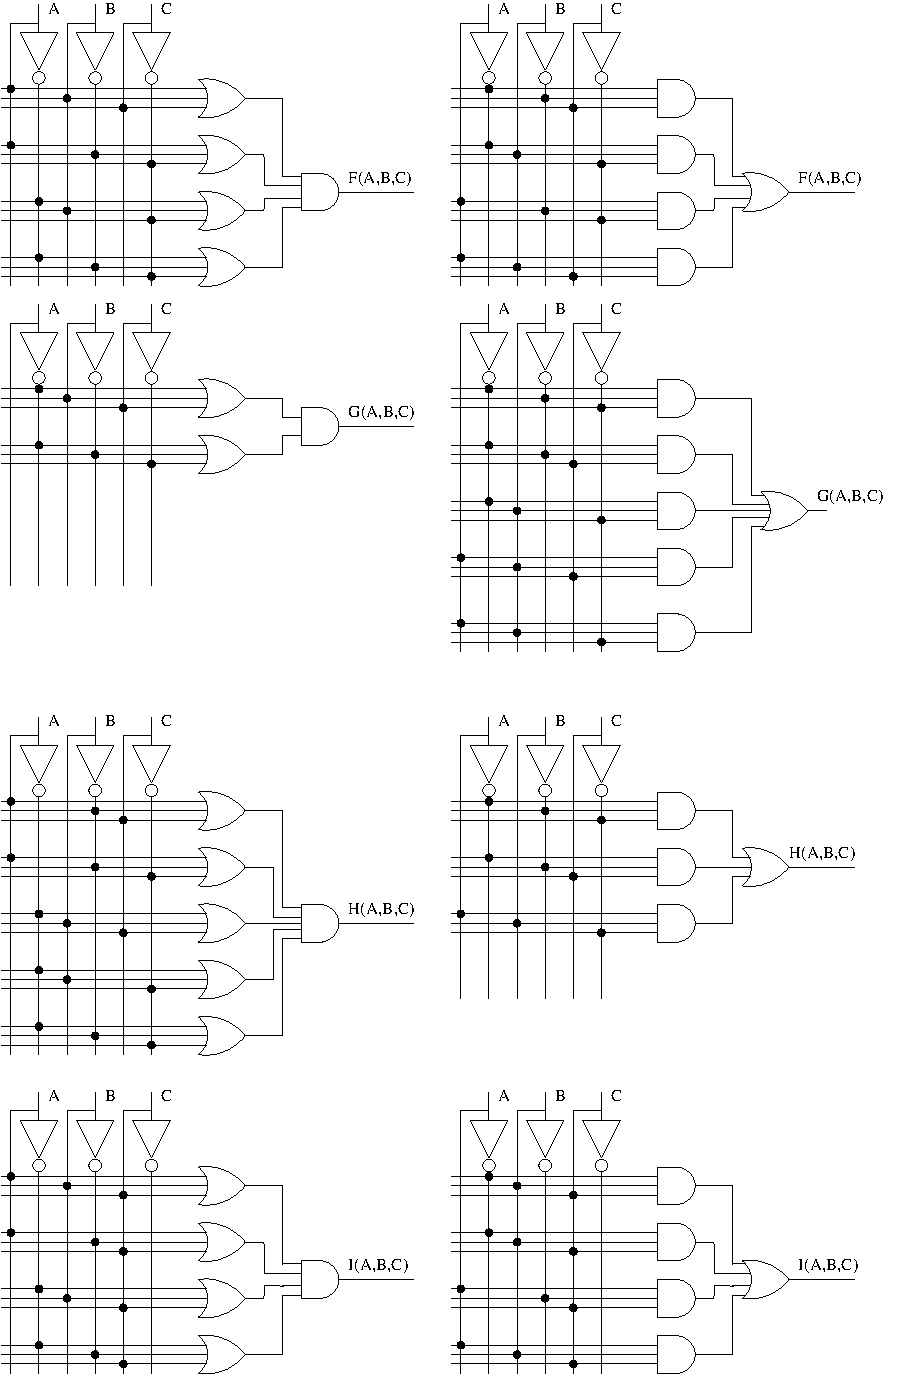
\includegraphics{./FigHw2/Sol2-4}}
	\end{figure}
}\end{solution}
\end{enumerate}
Treat each output independently of the other.  For example when
working with function $I$, cover up the columns $F,G$ and $H$.

$$\begin{array}{c|c|c||c|c|c|c}
 	A & B & C & F & G & H & I \\ \hline
 	0 & 0 & 0 & 0 & 1 & 1 & 0 \\ \hline
 	0 & 0 & 1 & 1 & 1 & 1 & 1 \\ \hline
 	0 & 1 & 0 & 1 & 1 & 0 & 0 \\ \hline
 	0 & 1 & 1 & 0 & 1 & 0 & 1 \\ \hline
 	1 & 0 & 0 & 1 & 0 & 0 & 0 \\ \hline
 	1 & 0 & 1 & 0 & 1 & 0 & 1 \\ \hline
 	1 & 1 & 0 & 0 & 1 & 1 & 0 \\ \hline
 	1 & 1 & 1 & 1 & 0 & 0 & 1 \\
\end{array}$$

\item  {\bf (2 pts. each)} Prove the validity of the following 
statements using the laws of Boolean Algebra. For each step of 
the proof, identify which law was used.
\begin{enumerate}
	\item $X'Y' + XY + X'Y = X' + Y$

\begin{solution}{
\begin{tabular}{lr}
X'Y' + XY + X'Y = 	& 3D\\
X'Y' + X'Y + XY+ X'Y =	& 8 \\
X'(Y' + Y )+ Y(X+ X')Y=	& 5 \\
X' + Y 			& QED \\
\end{tabular} }\end{solution}

	\item $(X+Y')X'Y' = X'Y'$

\begin{solution}{
\begin{tabular}{lr}
(X+Y')X'Y' = 	& 8 \\
XX'Y + X'Y'Y' = & 5D \\
0+X'Y'= 	& 1 \\
X'Y' 		& QED \\
\end{tabular}}\end{solution}

	\item $(X+Y)(X'+Z) = XZ + X'Y$

\begin{solution}{
\begin{tabular}{lr}
(X+Y)(X'+Z) = 		& 8 \\
(X+Y)X' + (X+Y)Z = 	& 8 \\
XX' + YX' + XZ + YZ =	& 1D,5 \\
YX' + XZ + YZ(X+X') =  	& 8 \\
YX' + XZ + XYZ + X'YZ =	& 6  \\
X'Y + X'YZ + XZ + XYZ =	& 1D, 8 \\
X'Y(1+Z) + XZ(1+Y) =  	& 2, 1D \\
X'Y + XZ 		& QED \\
\end{tabular} }\end{solution}

	\item $X'Y' + (X+Y)Z = X'Y' + Z$

\begin{solution}{
\begin{tabular}{lr}
X'Y' + (X+Y)Z = 				& 8\\
X'Y' + XZ + YZ = 				& 1D,5 \\
X'Y'*(Z+Z') + XZ + YZ(X+X') =  			& 8 \\
X'Y'Z' + X'Y'Z + XZ + XYZ + X'YZ =  		& 3 \\
X'Y'Z' + X'Y'Z + X'Y'Z + XZ + XYZ + X'YZ =  	& 8 \\
X'Y'(Z+Z') + XZ(1+Y) + X'Z(Y'+Y) =  		& 5,1D \\
X'Y' + XZ + X'Z  =  				& 8 \\
X'Y' + Z(X+X') =  				& 5, 1D\\
X'Y' + Z 					& QED \\
\end{tabular} }\end{solution}

	\item $A'C+BC+AB = A'C+AB$

\begin{solution}{
\begin{tabular}{lr}
A'C + BC+AB =  					& 1D, 5 \\
A'C + (A+A')BC + AB(C+C') 			& 8  \\
A'C + ABC + A'BC + ABC + ABC'= 			& 3\\
A'C + A'BC + ABC + ABC'= 			& 8\\
A'C(1+B) + AB(C+C')= 				& 5, 1D\\
A'C + AB 					& QED \\
\end{tabular} }\end{solution}
	\item $A(B+C)=AB+AB'C$

\begin{solution}{
\begin{tabular}{lr}
AB+AB'C= 					& 1D,5\\
AB(C+C') + AB'C= 				& 8 \\
ABC+ABC'+AB'C= 					& 3 \\
ABC + ABC + ABC' + AB'C= 			& 6\\
ABC + ABC' + ABC + AB'C= 			& 8\\
AB(C+C'+C) + AB'C = 				& 8\\	
AB + AB'C= 					& QED\\
\end{tabular}	}\end{solution}
	\item $(A+B+C)(A+B+C')(A'+B+C')(A'+B'+C') = (A+B)(A'+C')$

\begin{solution}{
\begin{tabular}{lr}
(A+B+C)(A+B+C')(A'B+C')(A'+B'+C')= 		& 4\\
((A+B+C)(A+B+C')(A'B+C')(A'+B'+C'))''= 		& 9D\\
(A'B'C + A'B'C' + AB'C + ABC)'= 		& 8\\
(A'B'(C+C') + AC(B'+B))'= 			& 5, 1D\\
(A'B' + AC)'= 					& 9 \\
(A+B)(A'+C')= 					& QED \\
\end{tabular}	}\end{solution}
\end{enumerate}

\item {\bf (4 pts.)} Design a circuit called MUX2.  MUX2 has three bits 
of input $S, y_0, y_1$ and one bit of output $F$.  If $S=0$, then 
$F=y_0$; else if $S=1$, then $F=y_1$.
\begin{enumerate}
	\item Write down the truth table for the MUX2 function.

\begin{solution}{
	\begin{tabular}{l|l|l|l}
	S & y0 &  y1 & F \\ \hline
	0 & 0  &  0  & 0 \\ \hline
	0 & 0  &  1  & 0 \\ \hline
	0 & 1  &  0  & 1 \\ \hline
	0 & 1  &  1  & 1 \\ \hline
	1 & 0  &  0  & 0 \\ \hline
	1 & 0  &  1  & 1 \\ \hline
	1 & 1  &  0  & 0 \\ \hline
	1 & 1  &  1  & 1 \\ 
	\end{tabular}
}\end{solution}

	\item Determine the canonical SOP realization for MUX2; 
		do not simplify.

\begin{solution}{F = S'y0y1' + S'y0y1 + Sy0'y1 + Sy0y1}\end{solution}
\end{enumerate}

\item {\bf (6 pts.)} Design a circuit called MUX4.  MUX4 has six bits of input 
$S_1 S_0, y_0, y_1, y_2, y_3$ and one bit of output $F$.  \\
If      $S_1 S_0 = 00$ then $F=y_0$  \\
else if $S_1 S_0 = 01$ then $F=y_1$ \\
else if $S_1 S_0 = 10$ then $F=y_2$ \\
else if $S_1 S_0 = 11$ then $F=y_3$ \\
Without writing down the truth table determine a SOP expression
to realize F by listing all possible inputs which will cause F to equal 1.
Then try to simplify your expression using Boolean Algebra.

\begin{solution}{
The output F only equals one in the following cases.
\begin{description}
\item S1=0 S0=0 and y0=1
\item S1=0 S0=1 and y1=1
\item S1=1 S0=0 and y2=1
\item S1=1 S0=1 and y3=1
\end{description}

With this information we can form four product terms, one for each input, 
that equal 1 only for that input.  ORing together these product terms 
will give us the solution to the problem.

$F = S_1'S_0'y_0 + S_1'S_0 y_1 + S_1 S_0'y_2 + S_1 S_0 y_3$
} \end{solution}

\item  {\bf (4 pts.)} Design a logic circuit called {\it MAJ} which 
has three inputs $A,B,C$ and one output $Z$. The output equals 1 
when a majority of the inputs are equal to 1, otherwise the output is 0.
\begin{enumerate}
	\item Write the truth table for the MAJ function.

\begin{solution}{
	\begin{tabular}{l|l|l||l} \\ 
	A & B & C &  F \\ \hline
	0 & 0 & 0 &  0 \\ \hline
	0 & 0 & 1 &  0 \\ \hline
	0 & 1 & 0 &  0 \\ \hline
	0 & 1 & 1 &  1 \\ \hline
	1 & 0 & 0 &  0 \\ \hline
	1 & 0 & 1 &  1 \\ \hline
	1 & 1 & 0 &  1 \\ \hline
	1 & 1 & 1 &  1 \\ 
	\end{tabular}
}\end{solution}
	\item Determine the canonical SOP realization for the MAJ
	function, do not simplify.

\begin{solution}{ F = A'BC + AB'C+ABC'+ABC} \end{solution}
\end{enumerate}

\item {\bf (4 pts.)} Let $X$ and $Y$ each be 2-bit signals whose 
elements are $x_1 x_0$ and $y_1 y_0$ respectively.  Determine the 
$\sum m$ and $\prod M$ expression for a circuit whose 1-bit 
output $z$ is defined by the following statement.
\begin{verbatim}
	if (X == Y) then z = 1 else z =0
\end{verbatim}

\begin{solution}{
The truth table for the solution is shown below.
$$\begin{array}{c|c|c|c||c|c||c}
a_1 & a_0 & b_1 & b_0 & A  & B & z  \\ \hline
0 & 0 & 0 & 0 & 0 & 0 & 1  \\ \hline
0 & 0 & 0 & 1 & 0 & 1 & 0  \\ \hline
0 & 0 & 1 & 0 & 0 & 2 & 0  \\ \hline
0 & 0 & 1 & 1 & 0 & 3 & 0  \\ \hline
0 & 1 & 0 & 0 & 1 & 0 & 0  \\ \hline
0 & 1 & 0 & 1 & 1 & 1 & 1  \\ \hline
0 & 1 & 1 & 0 & 1 & 2 & 0  \\ \hline
0 & 1 & 1 & 1 & 1 & 3 & 0  \\ \hline
1 & 0 & 0 & 0 & 2 & 0 & 0  \\ \hline
1 & 0 & 0 & 1 & 2 & 1 & 0  \\ \hline
1 & 0 & 1 & 0 & 2 & 2 & 1  \\ \hline
1 & 0 & 1 & 1 & 2 & 3 & 0  \\ \hline
1 & 1 & 0 & 0 & 3 & 0 & 1  \\ \hline
1 & 1 & 0 & 1 & 3 & 1 & 0  \\ \hline
1 & 1 & 1 & 0 & 3 & 2 & 0  \\ \hline
1 & 1 & 1 & 1 & 3 & 3 & 1  \\
\end{array}$$

The solution is shown below.

$z = \sum m(0,5,10,15) = \prod M(1,2,3,4,6,7,8,9,11,12,13,14)$
} \end{solution}


\item {\bf (4 pts.)} Let $X$ and $Y$ each be 2-bit signals whose 
elements are $x_1 x_0$ and $y_1 y_0$, respectively.  Determine the 
$\sum m$ and $\prod M$ expressions for a circuit whose 1-bit
output $z$ is defined by the following statement.
\begin{verbatim}
        if (X + Y > 3) then z = 0 else z =1
\end{verbatim}

\begin{solution}{
The truth table for the problem is shown below
$$\begin{array}{c|c|c|c||c|c||c}
a_1 & a_0 & b_1 & b_0 & A  & B & z  \\ \hline
0 & 0 & 0 & 0 & 0 & 0 & 1  \\ \hline
0 & 0 & 0 & 1 & 0 & 1 & 1  \\ \hline
0 & 0 & 1 & 0 & 0 & 2 & 1  \\ \hline
0 & 0 & 1 & 1 & 0 & 3 & 1  \\ \hline
0 & 1 & 0 & 0 & 1 & 0 & 1  \\ \hline
0 & 1 & 0 & 1 & 1 & 1 & 1  \\ \hline
0 & 1 & 1 & 0 & 1 & 2 & 1  \\ \hline
0 & 1 & 1 & 1 & 1 & 3 & 0  \\ \hline
1 & 0 & 0 & 0 & 2 & 0 & 1  \\ \hline
1 & 0 & 0 & 1 & 2 & 1 & 1  \\ \hline
1 & 0 & 1 & 0 & 2 & 2 & 0  \\ \hline
1 & 0 & 1 & 1 & 2 & 3 & 0  \\ \hline
1 & 1 & 0 & 0 & 3 & 0 & 1  \\ \hline
1 & 1 & 0 & 1 & 3 & 1 & 0  \\ \hline
1 & 1 & 1 & 0 & 3 & 2 & 0  \\ \hline
1 & 1 & 1 & 1 & 3 & 3 & 0  \\
\end{array}$$
Leading to this answer
$ z = \sum m(0,1,2,3.4,5,6,8,12) = \prod M(7,9,10,11,13,14,15)$
}\end{solution}

	

\item {\bf (3 pts.)} Determine the canonical SOP and POS expression for 
$F(A,B,C) = \prod M (0,1,4,5)$  Hint, compose the truth table for $F$.

\begin{solution}{
F(A,B,C)=A'BC' + A'BC +ABC' +ABC  \\
F(A,B,C)=(A+B+C)(A+B+C')(A'+B+C)(A'+B+C')
}\end{solution}

\item {\bf (3 pts.)} Determine the canonical SOP and POS expression for 
$F(A,B,C,D) = \sum m(0,4,12,15)$ Hint, write out the truth table for $F$.

\begin{solution}{
F(A,B,C)=A'B'C'D' + A'BC'D' + ABC'D' + ABCD  \\
F(A,B,C)=(A+B+C+D')(A+B+C'+D)(A+B+C'+D') (A+B'+C+D')(A+B'+C'+D) \\
(A+B'+C'+D')(A'+B+C+D)(A'+B+C+D') (A'+B+C'+D)(A'+B+C'+D')(A'+B'+C+D')\\
(A'+B'+C'+D)
}\end{solution}

\item {\bf (4 pts.)} For the function $F(A,B,C)= BC+AB'C'$,  draw
a timing diagram for an input sequence that follows the same order 
as the rows of the truth table.  Assume a propagation delay for NOT, 
AND and OR gate are all 10nS.

	\begin{solution}{skipped for now}\end{solution}

\item {\bf (4 pts.)} Complete the timing diagram in Figure~\ref{fig:HWtime}
for the functions
$F(A,B,C) = AB' + BC + ABC'$ and $G(A,B,C) = (A+B')C + (BC')'$
\begin{figure}[ht]
\center{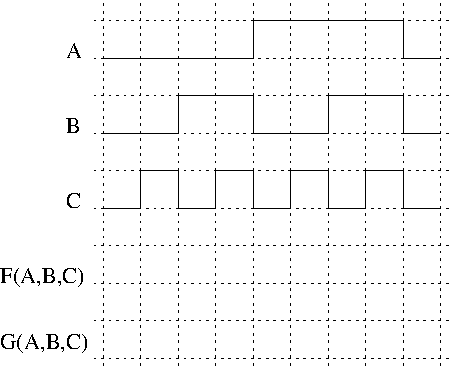
\includegraphics{./FigHw2/Prob2-14}}
\caption{The timing diagram for two functions, $F$ and $G$.}
\label{fig:HWtime}
\end{figure}

\begin{solution}{

\begin{figure}[ht]
\center{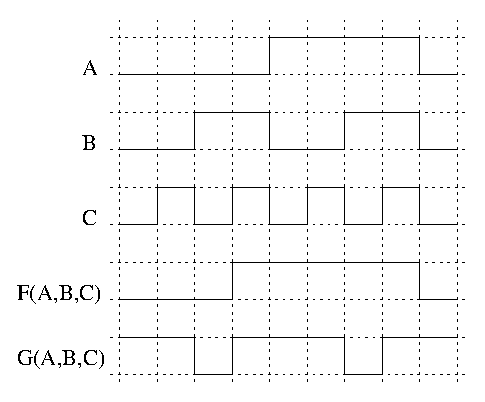
\includegraphics{./FigHw2/Sol2-14}}
\end{figure}
}\end{solution}

\item{\bf (16 pts.)} Design a circuit to control
the water pump of a washing machine.  The pump will not pump 
water if
\begin{description}
\item The lid is closed and the cycle is not fill
\item The cycle is fill and the detergent level is empty
\item The detergent is not empty and the lid is open
\end{description}
                                                                                
The variables for this problem are:
\begin{description}
\item L = lid is closed
\item C = cycle is fill
\item D = detergent is empty
\item P = pump will pump water
\end{description}
                                                                                
                                                                                
Create a truth table which describes when the pump will not
pump water.  Call this output P'.  Determine the canonical SOP
expression for P'.  Use this canonical SOP expression to generate
a circuit diagram for P.  This can be done by inserting an
inverter onto the output of the circuit.
                                                                                
Take the P' column from truth table and invert all the entries
to generate a new output column called P (because
the negation of P' is P).  Determine the canonical SOP
realization for P using this new column.
\end{enumerate}


\chapter{Minimization of Logical Functions}
\begin{enumerate}
\item {\bf (6 pts.)} Design a circuit called DECODE.  DECODE has two bits of 
input $S, D$ and two bit of output $y_1 y_0$.  If $S=0$ then $y_0=D$ and 
$y_1=0$ else if $S=1$ then $y_0=0$ and $y_1 = D$.
\begin{enumerate}
        \item Write down the truth table for the DECODE function.


\begin{solution}{
	\begin{tabular}{l|l||l|l}
	S & D & $y_1$ & $y_0$ \\ \hline
	0 & 0 & 0   & 0   \\ \hline
	0 & 1 & 0   & 1   \\ \hline
	0 & 0 & 0   & 0   \\ \hline
	1 & 1 & 1   & 0   \\ 
	\end{tabular}
} \end{solution}
        \item Determine the \SOPmin realization for DECODE.


\begin{solution}{
$y_0 = S'D$\\
$y_1 = S D$
} \end{solution}
\end{enumerate}

\item {\bf (6 pts.)} Design a circuit called FULLADD.  FULLADD has 
three bits of input $a,b,c$ and two bits of output $s_1 s_0$.  The output 
represents the sum of the three bits.
\begin{enumerate}
        \item Write down the truth table for the FULLADD function.


\begin{solution}{
	\begin{tabular}{l|l|l|l|l}
	a & b & c & $s_1$ & $s_0$ \\ \hline
	0 & 0 & 0 & 0   & 0   \\ \hline
	0 & 0 & 1 & 0   & 1   \\ \hline
	0 & 1 & 0 & 0   & 0   \\ \hline
	0 & 1 & 1 & 1   & 1   \\ \hline
	1 & 0 & 0 & 0   & 0   \\ \hline
	1 & 0 & 1 & 1   & 1   \\ \hline
	1 & 1 & 0 & 1   & 0   \\ \hline
	1 & 1 & 1 & 1   & 1   \\ 
\end{tabular}
} \end{solution}
        \item Determine the \SOPmin realization for FULLADD.

\begin{solution}{
$s_1 = ab + ac + bc $ \\
$s_0 = a'b'c + a'bc' + ab'c' + abc $
} \end{solution}
\end{enumerate}

\item  {\bf (4 pts.)} Determine \SOPmin expression for the following circuit
and draw the circuit using the fewest number of gates possible.
\begin{figure}[ht]
%% scalebox
\center{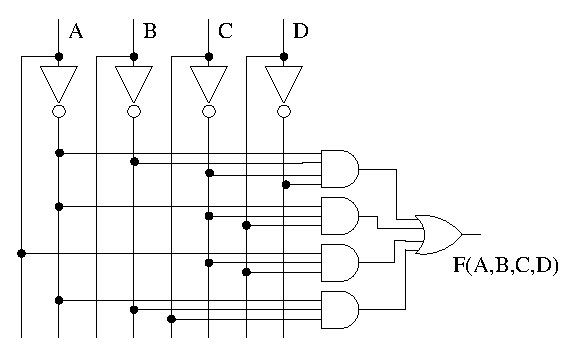
\includegraphics{./FigHw3/Prob3-3}}
\label{fig:Hw3}
\end{figure}

\begin{solution}{
From the circuit we have:
F(A,B,C,D) = A'B'C'D' + A'C'D + AC'D + A'B'C
$$ \begin{array} {c||c|c|c|c}
       AB \bs CD & 00 & 01 & 11 & 10 \\ \hline \hline
       00        & 1  & 1  & 1  & 1  \\ \hline
       01        &    & 1  &    &    \\ \hline
       11        &    & 1  &    &    \\ \hline
       10        &    & 1  &    &    \\
\end{array} $$ 
From this it follows that 
F(A,B,C,D) =  A'B' + C'D
} \end{solution}

\item  {\bf (8 pts.)} Design a digital system with four bits of inputs 
$I_3 I_2 I_1 I_0$ and two bits of outputs $O_1 O_0$.  At least one
of the inputs is always equal to 1.  The output encodes the 
index of the most significant 1 in the input.
For example, if $I_3 I_2 I_1 I_0 = 0101$, then the index
of the most significant 1 is 2, hence $O_1 O_0 = 10$.  Submit:
\begin{itemize}
\item The truth table.

\begin{solution}{
	\begin{tabular}{l|l|l|l||l|l}
	$I_3$ & $I_2$ & $I_1$ & $I_0$ & $O_1$ & $O_0$ \\ \hline
	0 & 0 & 0 & 0 &  x & x \\ \hline
	0 & 0 & 0 & 1 &  0 & 0 \\ \hline
	0 & 0 & 1 & 0 &  0 & 1 \\ \hline
	0 & 0 & 1 & 1 &  0 & 1 \\ \hline
	0 & 1 & 0 & 0 &  1 & 0 \\ \hline
	0 & 1 & 0 & 1 &  1 & 0 \\ \hline
	0 & 1 & 1 & 0 &  1 & 0 \\ \hline
	0 & 1 & 1 & 1 &  1 & 0 \\ \hline
	1 & 0 & 0 & 0 &  1 & 1 \\ \hline
	1 & 0 & 0 & 1 &  1 & 1 \\ \hline
	1 & 0 & 1 & 0 &  1 & 1 \\ \hline
	1 & 0 & 1 & 1 &  1 & 1 \\ \hline
	1 & 1 & 0 & 0 &  1 & 1 \\ \hline
	1 & 1 & 0 & 1 &  1 & 1 \\ \hline
	1 & 1 & 1 & 0 &  1 & 1 \\ \hline
	1 & 1 & 1 & 1 &  1 & 1 \\ 
	\end{tabular}
} \end{solution}
\item \SOPmin expression for $O_1$ and $O_0$.

\begin{solution}{
\begin{tabular}{ll}
$ \begin{array} {c||c|c|c|c}
 I3 I2 \bs I1 I0 & 00 & 01 & 11 & 10 \\ \hline \hline
       00        & x  &    &    &    \\ \hline
       01        & 1  & 1  & 1  & 1  \\ \hline
       11        & 1  & 1  & 1  & 1  \\ \hline
       10        & 1  & 1  & 1  & 1  \\
\end{array} $ & 
$ \begin{array} {c||c|c|c|c}
 I3 I2 \bs I1 I0 & 00 & 01 & 11 & 10 \\ \hline \hline
       00        & x  &    & 1  & 1  \\ \hline
       01        &    &    &    &    \\ \hline
       11        & 1  & 1  & 1  & 1  \\ \hline
       10        & 1  & 1  & 1  & 1  \\
\end{array} $ \\
$O_1 = I_3 + I_2$ & $O_0=I_3 + I_2'I_1$ \\
\end{tabular}
} \end{solution}
\end{itemize}

\item {\bf (8 pts.)}
Design a 4-input $a_1 a_0 b_1 b_0$, 4 -output $O_3 O_2 O_1 O_0$
digital system.  $A=a_1 a_0$ and $B=b_1 b_0$ represent 2-bit binary
numbers.  The output should be the product (multiplication) of the inputs, 
that is $O = A*B$.  In addition to determining the output, determine the
number of bits of output. Submit:
\begin{itemize}
\item Truth tables.

\begin{solution}{
\begin{tabular}{l|l|l|l||l|l|l|l}
$a_1$ & $a_0$ & $b_1$ & $b_0$ & $O_3$ & $O_2$ & $O_1$ & $O_0$ \\ \hline
0&0&0&0 &0&0&0&0 \\ \hline
0&0&0&1 &0&0&0&0 \\ \hline
0&0&1&0 &0&0&0&0 \\ \hline
0&0&1&1 &0&0&0&0 \\ \hline
0&1&0&0 &0&0&0&0 \\ \hline
0&1&0&1 &0&0&0&1 \\ \hline
0&1&1&0 &0&0&1&0 \\ \hline
0&1&1&1 &0&0&1&1 \\ \hline
1&0&0&0 &0&0&0&0 \\ \hline
1&0&0&1 &0&0&1&0 \\ \hline
1&0&1&0 &0&1&0&0 \\ \hline
1&0&1&1 &0&1&1&0 \\ \hline
1&1&0&0 &0&0&0&0 \\ \hline
1&1&0&1 &0&0&1&1 \\ \hline
1&1&1&0 &0&1&1&0 \\ \hline
1&1&1&1 &1&0&0&1 \\
\end{tabular}
} \end{solution}

\item Minimal SOP expression for the outputs.

\begin{solution}{
\begin{tabular}{ll}
$\begin{array} {c||c|c|c|c}
 a1 a0 \bs b1 b0 & 00 & 01 & 11 & 10 \\ \hline \hline
       00        &    &    &    &    \\ \hline
       01        &    &    &    &    \\ \hline
       11        &    &    & 1  &    \\ \hline
       10        &    &    &    &    \\
\end{array}$ &
$\begin{array} {c||c|c|c|c}
 a1 a0 \bs b1 b0 & 00 & 01 & 11 & 10 \\ \hline \hline
       00        &    &    &    &    \\ \hline
       01        &    &    &    &    \\ \hline
       11        &    &    &    & 1  \\ \hline
       10        &    &    & 1  & 1  \\
\end{array} $ \\
$O_3 = a_1a_0b_1b_0$ & $O_2 = a_1a_0'b_1 + a_1b_1b_0'$\\
\end{tabular}
} \end{solution}


\begin{solution}{
\begin{tabular}{ll}
$\begin{array} {c||c|c|c|c}
 a1 a0 \bs b1 b0 & 00 & 01 & 11 & 10 \\ \hline \hline
       00        &    &    &    &    \\ \hline
       01        &    &    & 1  & 1  \\ \hline
       11        &    & 1  &    & 1  \\ \hline
       10        &    & 1  & 1  &    \\
\end{array}$ &
$\begin{array} {c||c|c|c|c}
 a1 a0 \bs b1 b0 & 00 & 01 & 11 & 10 \\ \hline \hline
       00        &    &    &    &    \\ \hline
       01        &    & 1  & 1  &    \\ \hline
       11        &    & 1  & 1  &    \\ \hline
       10        &    &    &    &    \\
\end{array}$ \\
$O_1 = a_1b_1'b_0 + a_1a_0'b_0 + a_1'a_0b_1+a_0b_1b_0'$ & $O_0 = a_0b_0$ \\
\end{tabular}
} \end{solution}

\end{itemize}

\item  {\bf (8 pts.)}
Design a 4-bit Gray-code to binary converter.  A 4-bit gray-code is a 
sequence of 4-bit values where successive values differ by a single
bit.  For this problem use the sequence: 0000, 0001, 0011, 0010, 
0110, 0111, 0101, 0100, 1100, 1101, 1111, 1110, 1010, 1011, 1001, 
1000.  The index of the 4-bit gray code is its binary value.  For
example, the 4-bit gray code 0111 is at index 5, therefore when
presented with 0111 on its input, the converter should output 0101.
Submit:
\begin{itemize}
\item A truth table for the converter.

\begin{solution}{
\begin{tabular}{l|l|l|l||l|l|l|l}
$a_3$ & $a_2$ & $a_1$ & $a_0$ & $f_3$ & $f_2$ & $f_1$ & $f_0$ \\ \hline
0&0&0&0 &0&0&0&0 \\ \hline
0&0&0&1 &0&0&0&1 \\ \hline
0&0&1&0 &0&0&1&1 \\ \hline
0&0&1&1 &0&0&1&0 \\ \hline
0&1&0&0 &0&1&1&0 \\ \hline
0&1&0&1 &0&1&1&1 \\ \hline
0&1&1&0 &0&1&0&1 \\ \hline
0&1&1&1 &0&1&0&0 \\ \hline
1&0&0&0 &1&1&0&0 \\ \hline
1&0&0&1 &1&1&0&1 \\ \hline
1&0&1&0 &1&1&1&1 \\ \hline
1&0&1&1 &1&1&1&0 \\ \hline
1&1&0&0 &1&0&1&0 \\ \hline
1&1&0&1 &1&0&1&1 \\ \hline
1&1&1&0 &1&0&0&1 \\ \hline
1&1&1&1 &1&0&0&0 \\ 
\end{tabular}
} \end{solution}

\item Four k-maps for the converter.

\begin{solution}{
\begin{tabular}{ll}
$\begin{array} {c||c|c|c|c}
 a3 a2 \bs a1 a0 & 00 & 01 & 11 & 10 \\ \hline \hline
       00        &    &    &    &    \\ \hline
       01        &    &    &    &    \\ \hline
       11        & 1  & 1  & 1  & 1  \\ \hline
       10        & 1  & 1  & 1  & 1  \\
\end{array}$ &
$\begin{array} {c||c|c|c|c}
 a3 a2 \bs a1 a0 & 00 & 01 & 11 & 10 \\ \hline \hline
       00        &    &    &    &    \\ \hline
       01        & 1  & 1  & 1  & 1  \\ \hline
       11        &    &    &    &    \\ \hline
       10        & 1  & 1  & 1  & 1  \\
\end{array} $ \\
$f_3 = a_3$ & $f_2 = a_3a_2'+a_3'a_2$\\
\end{tabular}
} \end{solution}


\begin{solution}{
\begin{tabular}{ll}
$\begin{array} {c||c|c|c|c}
 a3 a2 \bs a1 a0 & 00 & 01 & 11 & 10 \\ \hline \hline
       00        &    &    & 1  & 1  \\ \hline
       01        & 1  & 1  &    &    \\ \hline
       11        & 1  & 1  &    &    \\ \hline
       10        &    &    & 1  & 1  \\
\end{array}$ &
$\begin{array} {c||c|c|c|c}
 a3 a2 \bs a1 a0 & 00 & 01 & 11 & 10 \\ \hline \hline
       00        &    & 1  &    & 1  \\ \hline
       01        &    & 1  &    & 1  \\ \hline
       11        &    & 1  &    & 1  \\ \hline
       10        &    & 1  &    & 1  \\
\end{array}$ \\
$f_1 = a_2a_1'+a_2'a_1$ & $f_0 = a_1'a_0+a_1a_0'$ \\
\end{tabular}
} \end{solution}

\item \SOPmin expression for the outputs, no product sharing please
(use the \verb+-Dso+ command line option).
\item Espresso file for the converter
\item Espresso output in PLA format
\item Compare the number of gates required in your solution
versus the number of gates required by Espresso.
\end{itemize}

\item {\bf (4 pts. each)} Determine \SOPmin expression for:
\begin{enumerate}
\item $F(A,B,C)=\sum m(0,1,3,4,5)$

\begin{solution}{
$\begin{array} {c||c|c|c|c}
   A   \bs B C  & 00 & 01 & 11 & 10 \\ \hline \hline
       0        &  1 & 1  & 1  &    \\ \hline
       1        &  1 & 1  &    &    \\ 
\end{array}$ \\
F(A,B,C)= B'+A'C
} \end{solution}
\item $F(A,B,C,D)=\sum m(1,5,6,7,11,12,13,15)$

\begin{solution}{
$\begin{array} {c||c|c|c|c}
   A B \bs C D   & 00 & 01 & 11 & 10 \\ \hline \hline
       00        &    & 1  &    &    \\ \hline
       01        &    & 1  & 1  & 1  \\ \hline
       11        & 1  & 1  & 1  &    \\ \hline
       10        &    &    & 1  &    \\
\end{array}$  \\
F(A,B,C)= ABC'+A'C'D+ACD+A'BC
} \end{solution}
\item $F(A,B,C,D)=\sum m(0,2,5,6,8,11,12,13,14,15)$

\begin{solution}{
$\begin{array} {c||c|c|c|c}
   A B \bs C D   & 00 & 01 & 11 & 10 \\ \hline \hline
       00        & 1  &    &    & 1  \\ \hline
       01        &    & 1  &    & 1  \\ \hline
       11        & 1  & 1  & 1  & 1  \\ \hline
       10        & 1  &    & 1  &    \\
\end{array}$  \\
F(A,B,C,D) =  AB + BC'D + ACD + B'C'D' + A'CD'
} \end{solution}
\item $F(A,B,C,D,E)=\sum m(0,8,9,10,13,15,22,26,29,30,31)$

\begin{solution}{
\begin{tabular}{cc}
$\begin{array} {c||c|c|c|c}
   B C \bs D E   & 00 & 01 & 11 & 10 \\ \hline \hline
       00        & 1  &    &    &    \\ \hline
       01        &    &    &    &    \\ \hline
       11        &    & 1  & 1  &    \\ \hline
       10        & 1  & 1  &    & 1  \\
\end{array}$ &
$\begin{array} {c||c|c|c|c}
   B C \bs D E   & 00 & 01 & 11 & 10 \\ \hline \hline
       00        &    &    &    &    \\ \hline
       01        &    &    &    & 1  \\ \hline
       11        &    & 1  & 1  & 1  \\ \hline
       10        &    &    &    & 1  \\
\end{array}$ \\
A=0 & A=1 \\
\end{tabular} \\
F(A,B,C,D,E) = BCE + A'C'D'E' + BC'DE + ACDE' + A'BD'E or \\
F(A,B,C,D,E) = BCE + A'C'D'E' + BC'DE + ACDE' + A'BC'D'
} \end{solution}

\item $F(A,B,C,D,E)=\sum m(0,2,4,5,7,10,13,15,18,21,24,26,28,29)$

\begin{solution}{
\begin{tabular}{cc}
$\begin{array} {c||c|c|c|c}
   B C \bs D E   & 00 & 01 & 11 & 10 \\ \hline \hline
       00        & 1  &    &    & 1  \\ \hline
       01        & 1  & 1  & 1  &    \\ \hline
       11        &    & 1  & 1  &    \\ \hline
       10        &    &    &    & 1  \\
\end{array}$ &
$\begin{array} {c||c|c|c|c}
   B C \bs D E   & 00 & 01 & 11 & 10 \\ \hline \hline
       00        &    &    &    & 1  \\ \hline
       01        &    & 1  &    &    \\ \hline
       11        & 1  & 1  &    &    \\ \hline
       10        & 1  &    &    & 1  \\
\end{array}$ \\
A=0 & A=1 \\
\end{tabular} \\
F(A,B,C,D,E) = A'B'D'E' + CD'E+C'DE'+ABD'E'+A'CE
} \end{solution}

\end{enumerate}

\item {\bf (4 pts. each)} Determine \SOPmin expression for:
\begin{enumerate}
\item $F(A,B,C,D)=\sum m(4,7,9,12,13,15)+\sum d(0,1,2,3,10,14)$

\begin{solution}{
$\begin{array} {c||c|c|c|c}
   A B \bs C D   & 00 & 01 & 11 & 10 \\ \hline \hline
       00        & x  & x  & x  &    \\ \hline
       01        & 1  &    & 1  &    \\ \hline
       11        & 1  & 1  & 1  & x  \\ \hline
       10        &    & 1  &    & x  \\
\end{array}$  \\
F(A,B,C,D) = BC'D'+AC'D+BCD
} \end{solution}

\item $F(A,B,C,D)=\sum m(0,1,5,7,10,14,15)+\sum d(2,8)$

\begin{solution}{
$\begin{array} {c||c|c|c|c}
   A B \bs C D   & 00 & 01 & 11 & 10 \\ \hline \hline
       00        & 1  & 1  &    & x  \\ \hline
       01        &    & 1  & 1  &    \\ \hline
       11        &    &    & 1  & 1  \\ \hline
       10        & x  &    &    & 1  \\
\end{array}$ \\
F(A,B,C,D) = B'D'+A'C'D+BCD+ABC
} \end{solution}
\item $F(A,B,C,D)=\sum m(0,1,3,4,15)+\sum d(10,12)$

\begin{solution}{

$\begin{array} {c||c|c|c|c}
   A B \bs C D   & 00 & 01 & 11 & 10 \\ \hline \hline
       00        & 1  & 1  & 1  &    \\ \hline
       01        & 1  &    &    &    \\ \hline
       11        & x  &    & 1  &    \\ \hline
       10        &    &    &    & x  \\
\end{array}$ \\
F(A,B,C,D)=ABCD+A'C'D'+A'B'D
} \end{solution}
\item $F(A,B,C,D,E)=\sum m(2,3,5,7,11,13,17,19,29,31)+\sum d(1,4,9,16,25)$

\begin{solution}{

\begin{tabular}{cc}
$\begin{array} {c||c|c|c|c}
   B C \bs D E   & 00 & 01 & 11 & 10 \\ \hline \hline
       00        &    & x  & 1  & 1  \\ \hline
       01        & x  & 1  & 1  &    \\ \hline
       11        &    & 1  &    &    \\ \hline
       10        &    & x  & 1  &    \\
\end{array}$ &
$\begin{array} {c||c|c|c|c}
   B C \bs D E   & 00 & 01 & 11 & 10 \\ \hline \hline
       00        & x  & 1  & 1  &    \\ \hline
       01        &    &    &    &    \\ \hline
       11        &    & 1  & 1  &    \\ \hline
       10        &    & x  &    &    \\
\end{array}$ \\
A=0 & A=1 \\
\end{tabular} \\
F(A,B,C,D,E)=A'D'E+A'C'E+A'B'C'D+B'C'E+ABCE +A'B'E
} \end{solution}

\item $F(A,B,C,D,E)=\sum m(2,3,6,10,12,13,14,18,25,26,28,29)+\sum d(11,27)$

\begin{solution}{

\begin{tabular}{cc}
$\begin{array} {c||c|c|c|c}
   B C \bs D E   & 00 & 01 & 11 & 10 \\ \hline \hline
       00        &    &    & 1  & 1  \\ \hline
       01        &    &    &    & 1  \\ \hline
       11        & 1  & 1  &    & 1  \\ \hline
       10        &    &    & x  & 1  \\
\end{array}$ &
$\begin{array} {c||c|c|c|c}
   B C \bs D E   & 00 & 01 & 11 & 10 \\ \hline \hline
       00        &    &    &    & 1  \\ \hline
       01        &    &    &    &    \\ \hline
       11        & 1  & 1  &    &    \\ \hline
       10        &    & 1  & x  & 1  \\
\end{array}$ \\
A=0 & A=1 \\
\end{tabular} \\
F(A,B,C,D,E)=A'C'D+C'DE'+A'DE' +BCD' + ABC'E 
} \end{solution}

\end{enumerate}

\item {\bf (8 pts. each)} Determine \SOPmin and \POSmin expressions for:
\begin{enumerate}
\item  $F(A,B,C,D) = \sum m(0,1,2,5,8,10,13,15)$

\begin{solution}{

\begin{tabular}{cc}
$\begin{array} {c||c|c|c|c}
   A B \bs C D   & 00 & 01 & 11 & 10 \\ \hline \hline
       00        & 1  & 1  &    & 1  \\ \hline
       01        &    & 1  &    &    \\ \hline
       11        &    & 1  & 1  &    \\ \hline
       10        & 1  &    &    & 1  \\
\end{array}$ &
$\begin{array} {c||c|c|c|c}
   A B \bs C D   & 00 & 01 & 11 & 10 \\ \hline \hline
       00        &    &    & 1  &    \\ \hline
       01        & 1  &    & 1  & 1  \\ \hline
       11        & 1  &    &    & 1  \\ \hline
       10        &    & 1  & 1  &    \\
\end{array}$ \\
F  & F' \\
\end{tabular} \\
\SOPmin F(A,B,C,D) =  B'D'+A'C'D+ABD\\
\POSmin F(A,B,C,D) =  (B'+D)(A+C'+D')(A'+B+D')
} \end{solution}

\item  $F(A,B,C,D) = \prod M(0,4,6,10,11,12)$

\begin{solution}{

\begin{tabular}{cc}
$\begin{array} {c||c|c|c|c}
   A B \bs C D   & 00 & 01 & 11 & 10 \\ \hline \hline
       00        &    & 1  & 1  & 1  \\ \hline
       01        &    & 1  & 1  &    \\ \hline
       11        &    & 1  & 1  & 1  \\ \hline
       10        & 1  & 1  &    &    \\
\end{array}$ &
$\begin{array} {c||c|c|c|c}
   A B \bs C D   & 00 & 01 & 11 & 10 \\ \hline \hline
       00        & 1  &    &    &    \\ \hline
       01        & 1  &    &    & 1  \\ \hline
       11        & 1  &    &    &    \\ \hline
       10        &    &    & 1  & 1  \\
\end{array}$ \\
F  & F' \\
\end{tabular} \\
\SOPmin F(A,B,C,D) = AB'C'+A'B'C+ABC+C'D+A'D  or \\
\SOPmin F(A,B,C,D) = AB'C'+A'B'C+ABC+C'D+BD  or \\
\SOPmin F(A,B,C,D) = AB'C'+A'B'C+ABC+A'D+BD \\
\POSmin F(A,B,C,D) =  (A+C+D)(B'+C+D)(A+B'+D)(A'+B+C')
} \end{solution}
\item  $F(A,B,C,D) = \sum m(0,5,7,10,11,14) + \sum d(3,12,15)$

\begin{solution}{

\begin{tabular}{cc}
$\begin{array} {c||c|c|c|c}
   A B \bs C D   & 00 & 01 & 11 & 10 \\ \hline \hline
       00        & 1  &    & x  &    \\ \hline
       01        &    & 1  & 1  &    \\ \hline
       11        & x  &    & x  & 1  \\ \hline
       10        &    &    & 1  & 1  \\
\end{array}$ &
$\begin{array} {c||c|c|c|c}
   A B \bs C D   & 00 & 01 & 11 & 10 \\ \hline \hline
       00        &    & 1  & x  & 1  \\ \hline
       01        & 1  &    &    & 1  \\ \hline
       11        & x  & 1  & x  &    \\ \hline
       10        & 1  & 1  &    &    \\
\end{array}$ \\
F  & F' \\
\end{tabular} \\
\SOPmin F(A,B,C,D) =  A'B'C'D'+A'BD+AC\\
\POSmin F(A,B,C,D) =  (A'+C)(A+C'+D)(A+B+D')(B'+C+D) or \\ 
\POSmin F(A,B,C,D) =  (A'+C)(A+C'+D)(B+C+D')(B'+C+D) or \\ 
\POSmin F(A,B,C,D) =  (A'+C)(A+C'+D)(A+B+D')(A+B'+D) or \\ 
\POSmin F(A,B,C,D) =  (A'+C)(A+C'+D)(B+C+D')(A+B'+D)  \\ 
} \end{solution}
\item  $F(A,B,C,D) = \prod M(2,6,7,9,15) * \prod d(4,12,13) $

\begin{solution}{

\begin{tabular}{cc}
$\begin{array} {c||c|c|c|c}
   A B \bs C D   & 00 & 01 & 11 & 10 \\ \hline \hline
       00        & 1  & 1  & 1  &    \\ \hline
       01        & x  & 1  &    &    \\ \hline
       11        & x  & x  &    & 1  \\ \hline
       10        & 1  &    & 1  & 1  \\
\end{array}$ &
$\begin{array} {c||c|c|c|c}
   A B \bs C D   & 00 & 01 & 11 & 10 \\ \hline \hline
       00        &    &    &    & 1  \\ \hline
       01        & x  &    & 1  & 1  \\ \hline
       11        & x  & x  & 1  &    \\ \hline
       10        &    & 1  &    &    \\
\end{array}$ \\
F  & F' \\
\end{tabular} \\
\SOPmin F(A,B,C,D) =  A'C'+AD'+A'CD\\
\POSmin F(A,B,C,D) =  (A+C'+D)(B'+C'+D')(A'+C+D')
} \end{solution}
\item  $F(W,X,Y,Z) = WX'Z' + X'YZ + W'Y'Z + XYZ + WXY'$

\begin{solution}{
\begin{tabular}{cc}
$\begin{array} {c||c|c|c|c}
   W X \bs Y Z   & 00 & 01 & 11 & 10 \\ \hline \hline
       00        &    & 1  & 1  &    \\ \hline
       01        &    & 1  & 1  &    \\ \hline
       11        & 1  & 1  & 1  &    \\ \hline
       10        & 1  &    & 1  & 1  \\
\end{array}$ &
$\begin{array} {c||c|c|c|c}
   W X \bs Y Z   & 00 & 01 & 11 & 10 \\ \hline \hline
       00        & 1  &    &    & 1  \\ \hline
       01        & 1  &    &    & 1  \\ \hline
       11        &    &    &    & 1  \\ \hline
       10        &    & 1  &    &    \\
\end{array}$ \\
F  & F' \\
\end{tabular} \\
\SOPmin F(W,X,Y,Z) =  W'Z+XZ+WY'Z'+WX'Y\\
\POSmin F(W,X,Y,Z) = (W+Z)(X'+Y'+Z)(W'+X+Y+Z')
} \end{solution}

\item  $F(W,X,Y,Z) = (W + X'+Y')(W'+Z')(W+Y')$

\begin{solution}{

We have that $F'(W,X,Y,Z) = W'XY+ WZ+ W'Y$

\begin{tabular}{cc}
$\begin{array} {c||c|c|c|c}
   W X \bs Y Z   & 00 & 01 & 11 & 10 \\ \hline \hline
       00        &    &    & 1  & 1  \\ \hline
       01        &    &    & 1  & 1  \\ \hline
       11        &    & 1  & 1  &    \\ \hline
       10        &    & 1  & 1  &    \\
\end{array}$ &
$\begin{array} {c||c|c|c|c}
   W X \bs Y Z   & 00 & 01 & 11 & 10 \\ \hline \hline
       00        & 1  & 1  &    &    \\ \hline
       01        & 1  & 1  &    &    \\ \hline
       11        & 1  &    &    & 1  \\ \hline
       10        & 1  &    &    & 1  \\
\end{array}$ \\
F'  & F \\
\end{tabular} \\
\SOPmin F(W,X,Y,Z) =  W'Y'+WZ'\\
\POSmin F(W,X,Y,Z) = (W'+Z')(W+Y')
} \end{solution}
\end{enumerate}
Hint, the negation of a ``Don't care" is a ``Don't care".

\item {\bf (3 pts.)} While grading homework for a digital design class 
the following question/answer pair is encountered.  What is 
the problem with the answer given?

\begin{tabular}{l}
Question: Generate the \POSmin expression for $F(A,B,C) = \sum m(2,3,4,5)$ \\
Answer: $F(A,B,C) = (A+B')(A'+B)$ \\
\end{tabular}

\item {\bf (6 pts.)} Determine the \SOPmin realization of the following
function.

\begin{tabular}{c|c|c|c||c}
A & B & C & D & F(A,B,C,D) \\ \hline
x & 1 & 1 & x & 0 \\ \hline
0 & x & 0 & 1 & 0 \\ \hline
x & x & 0 & 0 & x \\ \hline
x & 0 & 1 & x & 1 \\ \hline
1 & x & 0 & 1 & 1 \\ 
\end{tabular}


\begin{solution}{
$\begin{array} {c||c|c|c|c}
   A B \bs B C   & 00 & 01 & 11 & 10 \\ \hline \hline
       00        & x  & 0  & 1  & 1  \\ \hline
       01        & x  & 0  & 0  & 0  \\ \hline
       11        & x  & 1  & 0  & 0  \\ \hline
       10        & x  & 1  & 1  & 1  \\
\end{array}$  \\
F(A,B,C) = AC'+B'C
} \end{solution}

\item {\bf (6 pts.)} What is the worst function \SOPmin of 3 variable 
that can be created?  That is, define a function whose minimal SOP form 
has the largest possible number of product terms.  What is the largest 
number of product terms that a 4-variable \SOPmin expression can 
have?  How about $N$ variables?

\begin{solution}{
The worst function of three variable is shown in the Kmap below:

$\begin{array} {c||c|c|c|c}
   A \bs B C   & 00 & 01 & 11 & 10 \\ \hline \hline
      0        & 1  &    & 1  &    \\ \hline
      1        &    & 1  &    & 1  \\ 
\end{array}$

This function requires four product terms.  Any additional minterm added to 
this Kmap would create a grouping with neighboring minterms, perhaps not 
decreasing the
the number of product terms, but certainly making the product terms simpler.
Its important to note that this configuration looks like a checkerboard.
The worst function of four variables looks like:

$\begin{array} {c||c|c|c|c}
   A B \bs B C   & 00 & 01 & 11 & 10 \\ \hline \hline
       00        & 1  &    & 1  &    \\ \hline
       01        &    & 1  &    & 1  \\ \hline
       11        & 1  &    & 1  &    \\ \hline
       10        &    & 1  &    & 1  \\
\end{array}$

This function requires 8 product terms, each containing every variable.  Boy that's
one bad realization.  In a general, the worst realization of an $N$ variable function 
requires $2^{N-1}$ product terms.  This is because the checkerboard configuration can
be applied to any Kmap, with half of the cells containing 1's.  Since a function with
$N$ variables has $2^{N}$ cells, then 1/2 of these cells works out to $2^{N-1}$.
} \end{solution} 


\item {\bf (16 pts.)} Sometimes a logic circuit needs to output 
a logic 0 in order to produce some behavior.  For example, an LED can be
attached to a digital circuit output so that it lights up when the circuit
outputs a 0.  This response is called an active low output; the output
device is {\it active} then the digital output is {\it low}.
                                                                                
Build a digital circuit that takes as input two 2-bit numbers,
A and B.  The circuit has three outputs which drive three
LEDs labeled G, L, and E.
The G LED should be illuminated when A$>$B.
The L LED should be illuminated when A$<$B.
The E LED should be illuminated when A=B.
The LEDs are illuminated when the circuit outputs a 0, otherwise
they are turned off.
                                                                                
Determine \SOPmin expression for the G, L and E outputs.
Determine \POSmin expression for the G, L and E outputs.
                                                                                


\end{enumerate}


\chapter{Combinational Logic Building Blocks}
\begin{enumerate}
\item {\bf (2 pts. each)}Short answer:
\begin{enumerate}
        \item How many 3:8 decoders would it take to build a 9:512 decoder?

	\begin{solution}{A total of 73 decoders are required.  There are 512/8 = 64 on
	the output layer, 64/8 = 8 in the middle layer and 1 on the input.}\end{solution}
        \item How many AND gates are there in a $2^N$:1 mux?

	\begin{solution}{ Each input requires 1 AND gate, hence $2^N$ AND gates.} \end{solution}
        \item How many AND gates are there in a $2^N:1$ mux which is
                constructed out of 2:1 muxes?

	\begin{solution}{ A $2^N$ Mux requires the following number of 2:1 muxes: 
        $$ 2^N/2 + 2^N/4 + ... + 2^N/2^N = $$
        $$ 2^N(1/2 + 1/4 + ... + 1/2^N) = $$
        $$ 2^N(1-1/2^(N+1)) =  $$
        $$ 2^N - 1  $$
	Since each 2:1 mux contains 2 AND gates, the total number of AND gates is
	$2^(N+1) - 2$.
	} \end{solution}

        \item How many AND gates are there in a $2^N$:1 mux which is
                constructed out of $2^L$:1 muxes, assume that
                $2^N$ is an integer multiple of $2^L$?

	\begin{solution}{
	A $2^N$ Mux requires the following number of $2^L:1$ muxes:
        $$ 2^N/2^L + 2^N/2^(2L) + ... 2^N/2^(kL) $$
        $$ 2^N(1/2^L + 1/2^(2L) + ... 1/2^(kL)) $$
	Where $k = N/L$.  Each $2^L:1$ mux requires $2^L$ AND gates for its construction,
	so the number of AND gates is the product of the number of $2^L:1$ muxes and the
	number of AND gates in a single $2^L:1$ mux, or:
        $$ 2^N * 2^L(1/2^L + 1/2^(2L) + ... 1/2^(kL)) $$
        $$ 2^N (1 + 1/2 + ... 1/2^k) $$
        $$ 2^N (2-1/2^(k+1)) $$
        $$ 2^N (2-1/2^(N/L+1) $$
        $$ 2^(N+1) - 2^(N-N/L-1) $$
	} \end{solution}

\end{enumerate}

\item {\bf (6 pts.)}Determine the \SOPmin expression for each of the 
three outputs of a bit-slice of the comparator.

	\begin{solution}{
	The following five variable Kmap describes $E_{out}$

\begin{tabular}{cc}
$\begin{array} {c||c|c|c|c}
 L_{in} G_{in}  \bs x  y & 00 & 01 & 11 & 10 \\ \hline \hline
       		00       & x  & x  & x  &  x \\ \hline
       		01       & 0  & 0  & 0  &  0 \\ \hline
       		11       & x  & x  & x  &  x \\ \hline
       		10       & 0  & 0  & 0  &  0 \\
\end{array}$ 
&
$\begin{array} {c||c|c|c|c}
 L_{in} G_{in}  \bs x  y & 00 & 01 & 11 & 10 \\ \hline \hline
       		00       & 1  & 0  & 1  & 0  \\ \hline
       		01       & x  & x  & x  & x  \\ \hline
       		11       & x  & x  & x  & x  \\ \hline
       		10       & x  & x  & x  & x  \\
\end{array}$  \\
$E_{in}=0$ & $E_{in}=1$ \\
\multicolumn{2}{c}{$E_{out} = L_{in}'G_{in}'x'y' + L_{in}'G_{in}'xy $} \\
\end{tabular}

The following five variable Kmap describes $G_{out}$

\begin{tabular}{cc}
$\begin{array} {c||c|c|c|c}
 L_{in} G_{in}  \bs x  y & 00 & 01 & 11 & 10 \\ \hline \hline
       		00       & x  & x  & x  & x  \\ \hline
       		01       & 1  & 1  & 1  & 1  \\ \hline
       		11       & x  & x  & x  & x  \\ \hline
       		10       & 0  & 0  & 0  & 0  \\
\end{array}$ 
&
$\begin{array} {c||c|c|c|c}
 L_{in} G_{in}  \bs x  y & 00 & 01 & 11 & 10 \\ \hline \hline
       		00       & 0  & 0  & 0  & 1  \\ \hline
       		01       & x  & x  & x  & x  \\ \hline
       		11       & x  & x  & x  & x  \\ \hline
       		10       & x  & x  & x  & x  \\
\end{array}$  \\
$E_{in}=0$ & $E_{in}=1$ \\
\multicolumn{2}{c}{$G_{out} = G_{in} + L_{in}'xy'$} \\
\end{tabular}

The following five variable Kmap describes $L_{out}$

\begin{tabular}{cc}
$\begin{array} {c||c|c|c|c}
 L_{in} G_{in}  \bs x  y & 00 & 01 & 11 & 10 \\ \hline \hline
       		00       & x  & x  & x  & x  \\ \hline
       		01       & 0  & 0  & 0  & 0  \\ \hline
       		11       & x  & x  & x  & x  \\ \hline
       		10       & 1  & 1  & 1  & 1  \\
\end{array}$ 
&
$\begin{array} {c||c|c|c|c}
 L_{in} G_{in}  \bs x  y & 00 & 01 & 11 & 10 \\ \hline \hline
       		00       & 0  & 1  & 0  & 0  \\ \hline
       		01       & x  & x  & x  & x  \\ \hline
       		11       & x  & x  & x  & x  \\ \hline
       		10       & x  & x  & x  & x  \\
\end{array}$  \\
$E_{in}=0$ & $E_{in}=1$ \\
\multicolumn{2}{c}{$L_{out} = L_{in} + G_{in}'x'y$} \\
\end{tabular}
} \end{solution}

\item {\bf (2 pts.)}Show how to connect together four 4-bit comparators to
construct a 16-bit comparator.

	\begin{solution}{ Figure forthcoming} \end{solution}

\item {\bf (2 pts.)}Determine the circuitry for the overflow detection 
circuit for a 2's-complement adder subtractor.  See page~\pageref{page:Ovf}.

	\begin{solution}{
$\begin{array} {c||c|c} \\
 c_{in}  \bs c_{out} & 0 & 1 \\ \hline 
                0    &   & 1 \\ \hline
                1    & 1 &   \\
\end{array}$   \\
Thus $ovf = c_{in}' c_{out} + c_{in} c_{out}' =  c_{in} \oplus c_{out} $
} \end{solution}


\item {\bf (10 pts.)}Build a BCD to 7-Segment Display converter using 
Espresso.  

\index{bcd to 7-segment}
\label{page:7seg}
\begin{tabular}{|l|p{3.5in}|} \hline
Nomenclature:  & BCD to 7-segment converter                \\ \hline
Data Input:    & 4-bit vector $D=d_3 d_2 d_1 d_0$  \\ \hline
Data Output:   & 7-bit vector $Y=y_6 \ldots y_1 y_0$    \\ \hline
Control:       & none                                   \\ \hline
Status:        & none                                   \\ \hline
Behavior:      & The output drives a 7-segment display pattern
		 representing the BCD digit.  \\ \hline
\end{tabular}

A binary coded digit (BCD) is a 4-bit binary number that is constrained
to assume the values of 0-9. That is, 1010 ... 1111 are illegal BCD digits.

A 7-segment display is a box with seven inputs and seven output LED bars.  
Each input is wired to an LED bar that is illuminated when a 1 is applied 
to its input.
Each of the seven LED segments is numbered according to the pattern shown
on the left-hand side of Figure~\ref{fig:BCD}. 

\begin{figure}[ht]
\center{\scalebox{0.7}{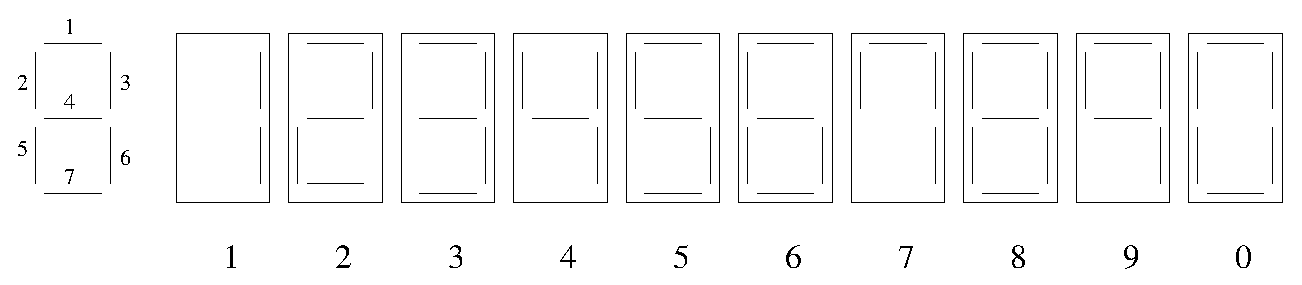
\includegraphics{./FigHw4/Prob4-5}}}
\caption{The numbering of the segments in a 7-segment display.
The patterns of the BCD digits.}
\label{fig:BCD}
\end{figure}

The pattern of LEDs to illuminate for each BCD digit is shown on the 
right-hand side of Figure~\ref{fig:BCD}.  A BCD to 7-segment converter 
has four inputs, $d_3 d_2 d_1 d_0$ and seven outputs $S_7 \ldots S_1$.  
Complete the design using Espresso.  Make sure to include ``Don't cares" 
in the truth table specification. 
\begin{enumerate}
	\item Use Espresso to determine the \SOPmin expression for the outputs 
	$S_7 \ldots S_1$.  Underline product terms that are shared.
	Submit the Espresso source file.

\begin{solution}{
The following is the source file for the BCD to 7-segment converter.

%% \begin{verbatim}
%% # BCD to 7-segment display
%% #
%% .i 4 
%% .o 7  
%% .ilb b3 b2 b1 b0  
%% .ob  s7 s6 s5 s4 s3 s2 s1 
%% 0000 1110111 
%% 0001 0100100 
%% 0010 1011101 
%% 0011 1101101 
%% 0100 0101110 
%% 0101 1101011 
%% 0110 1111011 
%% 0111 0100111 
%% 1000 1111111 
%% 1001 0101111 
%% 101- ------- 
%% 11-- -------  
%% .e  
%% \end{verbatim}

The following is the output from espresso on the 
BCD to 7-segment converter.

%% \begin{verbatim}
%% .i 4 
%% .o 7 
%% .ilb b3 b2 b1 b0 
%% .ob s7 s6 s5 s4 s3 s2 s1 
%% .p 9 
%% --11 0100100 
%% -00- 0100100 
%% -000 1010011 
%% --10 1011000 
%% -100 0101110 
%% -11- 0100011 
%% -101 1101011 
%% -01- 1001101 
%% 1--- 0001011 
%% .e 
%% \end{verbatim}
} \end{solution}

	\item Use Espresso to determine the \POSmin expression for the outputs 
	$S_7 \ldots S_1$.  Underline sum terms that are shared.
	Submit the Espresso source file
\begin{solution} {
The following output was generated by using the same file
as the solution in the previous part; but using the epos
option in espresso.

%% \begin{verbatim}
%% # BCD to 7-segment display 
%% # 
%% .i 4 
%% .o 7 
%% .ilb b3 b2 b1 b0 
%% .ob s7 s6 s5 s4 s3 s2 s1 
%% #.phase 0000000 
%% .p 9 
%% 000- 0001000 
%% -110 0000100 
%% -010 0100010 
%% -101 0010100 
%% 0001 1010011 
%% -011 0010010 
%% -100 1010001 
%% 1--1 1010000 
%% -111 1011000 
%% .e 
%% \end{verbatim}

Remember that these are the negation of the output variables, hence
we have to use DeMorgan's to put them into \POSmin form.  
Symbolically we have:
%% \begin{verbatim}
s7=(b3+b2+b1+b0')(b2'+b1+b0)(b3'+b0')(b2'+b1'+b0'); \\
s6=(b2+b1'+b0); \\
s5=(b2'+b1+b0')(b3+b2+b1+b0')(b2+b1+b0')(b2'+b1+b0)(b3'+b0')(b2'+b1'+b0'); \\
s4=(b3+b2+b1)(b2'+b1'+b0'); \\
s3=(b2'+b1'+b0)(b2'+b1+b0'); \\
s2=(b2+b1'+b0)(b3+b2+b1+b0')(b2+b1'+b0'); \\
s1=(b3+b2+b1+b0')(b2'+b1+b0); \\
%% \end{verbatim}
}\end{solution}
\end{enumerate}

\item {\bf (10 pts.)} Build a box which has one 4-bit input called A and  
one 4-bit output called T. The output T is the 2's-complement value
of the input A.  Use the bit slice paradigm to solve this
problem.  That is, create a building block for one bit of the problem 
then string four of them together to solve the problem.
For the problem at hand this can be done as follows:
\begin{enumerate}
	\item Start at the LSB of A.
        \item If this is the first, least significant, 1, flip all bits 
		to the left.
        \item If this is not the first 1, leave the bit alone.
        \item Move one bit to the left.
        \item Goto Step b.
\end{enumerate}
A bit-slice should communicate whether there has been a 1 to the right,
to the more significant bit.  Submit:
\begin{itemize}
	\item How the above "algorithm" behaves when presented with
        the inputs A=1100
        \item The truth table for one bit slice
        \item \SOPmin expression and circuit diagram for a bit slice.
        \item The organization of four bit slices to solve the problem
\end{itemize}

\begin{solution}{
	The key to the begin solution  is to figure out the structure
	of the begin solution  and then give meaning to the signals involved.
	The problem will be sliced into four bit-slices; each handled
	but its own complement box.  Thus, there will be four complement
	box in the begin solution.  Each box will have 2 inputs, one being
	a bit of A and the other being a "carry in" from the less
	significant less, immediately to the right.  Each box
	will have two bits of output, a bit of T and a "carry out".
	The carry bits (both into and out of a box will convey
	information regarding the rightmost 1 in the number A.

	If the carry in is equal 1 then there is a one to the right. 
	If the carry in is equal 0 then there is not a one to the right. 
	The truth table for a box is then

	\begin{table}
	\begin{tabular}{l|l||l|l|l}
	$A$ & $c_{in}$  & $T$ & $c_{out}$ & comment \\ \hline
	0   & 0   	&   0 & 0    	  & There is no 1 to the right \\ \hline
	0   & 1   	&   1 & 1    	  & There is a 1 to the right, flip A \\ \hline
	1   & 0   	&   1 & 1    	  & There is is no 1 to the right, but we've created one \\ \hline
	1   & 1   	&   0 & 1    	  & There is a 1 to the right, flip A \\ 
	\end{tabular}
	\end{table}

	From this it follows that: \\
	$T=A'c_{in} + A c_{in}'=A \oplus c_{in}$ \\
	$c_{out} = A + c_{in}$
}\end{solution}

\item {\bf (4 pts.)} Build a 7:128 decoder using a minimum number of 
4:16, 2:4 and 1:2 decoders. Describe the wiring of the select lines.
\begin{solution} {

\begin{figure}[ht]
\center{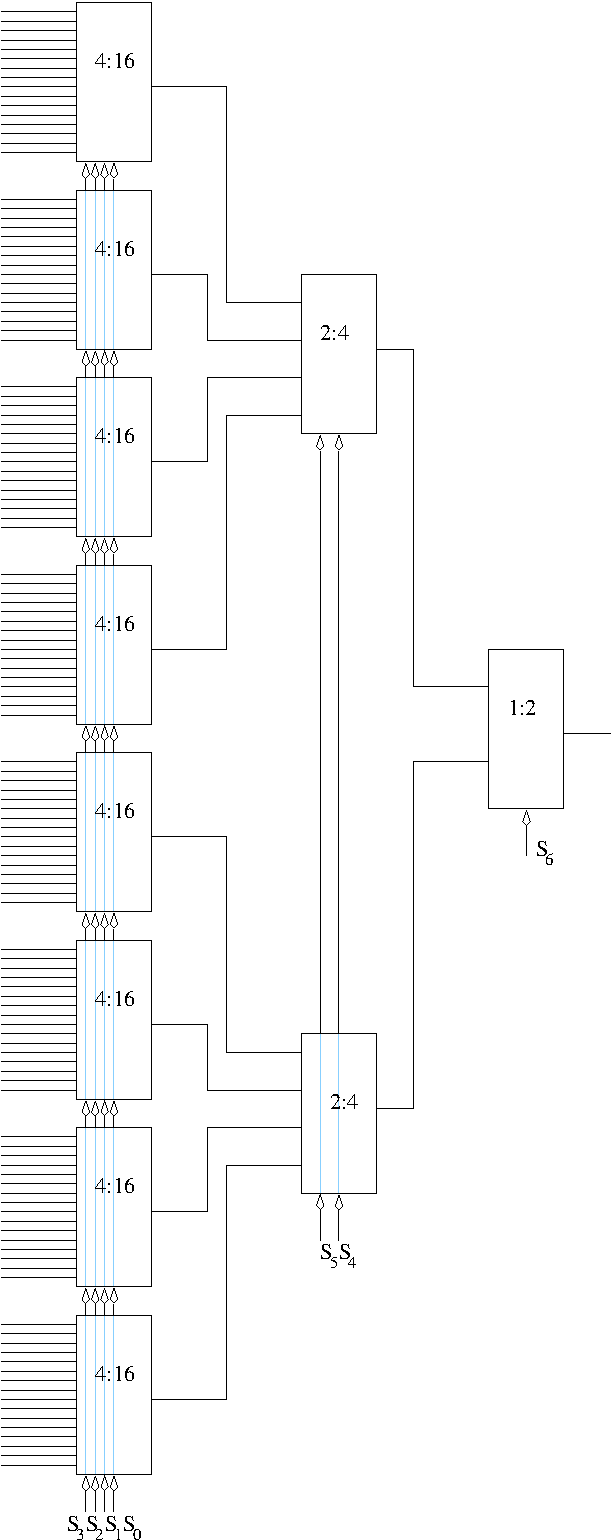
\includegraphics{./FigHw4/Sol4-7}}
\caption{A 7:128 decoder built from 4:16, 2:4 and 1:2 decoders.}
\label{fig:bighwdec}
\end{figure}
} \end{solution}



\item {\bf (4 pts. each)} Design a circuit with two 8-bit inputs $X,Y$, an 
8-bit output $Z$ and a 1-bit input $sel$.  Construct a circuit that yields the 
correct value of $Z$ using only the basic building blocks presented in this 
chapter; do NOT show the internal organization of these building blocks.  If 
a mux is used, denote which input is the $y_0$ and which is $y_1$.  
If a comparator is used denote which input is $X$ and which is $Y$.
Do not use any AND or OR gates; it will tempting in the later problems.
\begin{enumerate}
\item \verb^ if (sel==0) then Z = X else Z = Y ^

\begin{solution}{ 
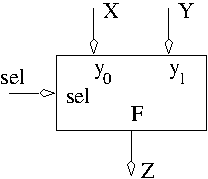
\includegraphics{./FigHw4/Sol4-8a}
} \end{solution}

\item \verb^ if (sel==0) then Z = X+Y else Z = Y ^

\begin{solution}{ 
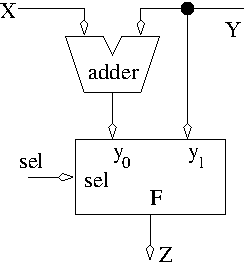
\includegraphics{./FigHw4/Sol4-8b}
} \end{solution}

\item \verb^ if (sel==0) then Z = X+Y else Z = X-Y ^

\begin{solution}{
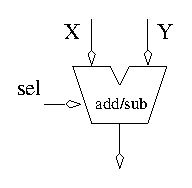
\includegraphics{./FigHw4/Sol4-8c}
} \end{solution}

\item \verb^ if (X==0) then Z = X else Z = Y ^

\begin{solution}{
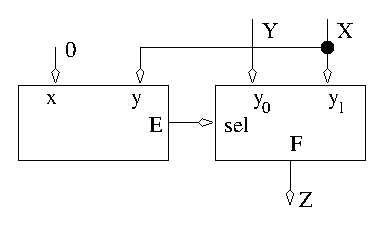
\includegraphics{./FigHw4/Sol4-8d}
} \end{solution}

\item \verb^ if (X==Y) then Z = X-Y else Z = Y ^

\begin{solution}{
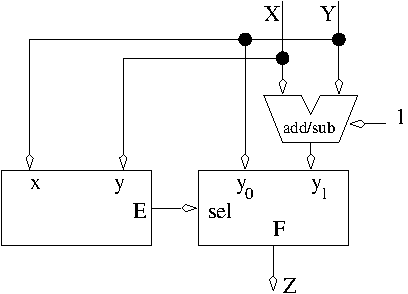
\includegraphics{./FigHw4/Sol4-8e}
} \end{solution}

\item \verb^ if (X==Y) then Z = X+Y else Z = X-Y ^

\begin{solution}{
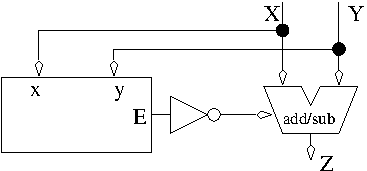
\includegraphics{./FigHw4/Sol4-8f}
} \end{solution}

\item \verb^ if (X < Y) then Z = X else Z = Y ^

\begin{solution}{
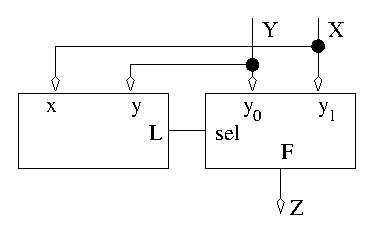
\includegraphics{./FigHw4/Sol4-8g}
} \end{solution}

\item \verb^ if (X <= Y) then Z = X else Z = Y ^

\begin{solution}{
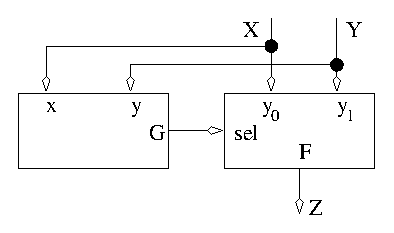
\includegraphics{./FigHw4/Sol4-8h}
} \end{solution}

\item \verb^ if (X > Y) then Z = X else Z = Y ^

\begin{solution}{
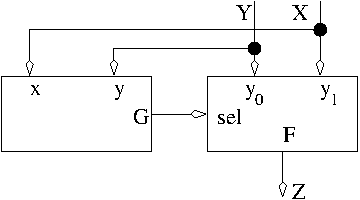
\includegraphics{./FigHw4/Sol4-8i}
} \end{solution}

\item \verb^ if (X > Y) then Z = X+X else Z = Y+Y ^

\begin{solution}{
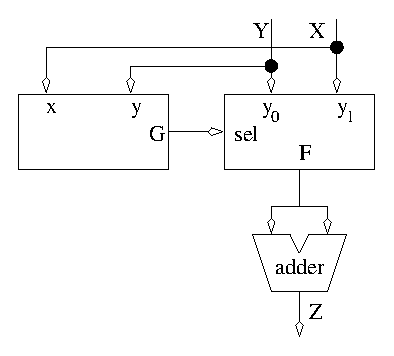
\includegraphics{./FigHw4/Sol4-8j}
} \end{solution}

\end{enumerate}

\item {\bf (10 pts.)} Build a 4-bit priority encoder.

\index{priority encoder}
\begin{tabular}{|l|p{3.5in}|} \hline
Nomenclature:  & N-bit priority encoder                \\ \hline
Data Input:    & N-bit vectored  $D=d_{N-1} \ldots d_1 d_0$  \\ \hline
Data Output:   & $\log_2(N)$-bit vector $Y=y_{log_2(N)} \ldots y_1 y_0$    \\ \hline
Control:       & none					\\ \hline
Status:        & none                                   \\ \hline
Behavior:      & $F = i$ where $i$ is the highest indexed input
			which equals 1.  When all inputs equal
			0, the output is a ``don't care".  \\ \hline
\end{tabular}
\label{page:prior}

The idea is for the outputs to represent (in binary code) the highest
input index which equals 1.  For example, a 4-bit priority encoder
with input $D=1010$ has inputs $d_3=1$ and $d_0=1$.  Of these two
inputs, the index of $d_3$ is greater than the index of $d_0$ so the
output, $F$ is equal to 3, or in binary $11$.  If the input were
$D=0111$ then $F=10$.

\begin{enumerate}
\item Write down the truth table for a 4-bit priority encoder.  Hint, 
the truth table could be structured so that it contains only five rows
by using ``don't cares" on the inputs.

\begin{solution}{
\begin{tabular}{l|l|l|l||l|l}
$d_3$ & $d_2$ & $d_1$ & $d_0$ & $f_1$ & $F_0$ \\ \hline
   0  &    0  &    0  &    0  &    x  &    x  \\ \hline
   0  &    0  &    0  &    1  &    0  &    0  \\ \hline
   0  &    0  &    1  &    x  &    0  &    1  \\ \hline
   0  &    1  &    x  &    x  &    1  &    0  \\ \hline
   1  &    x  &    x  &    x  &    1  &    1  \\
\end{tabular}
} \end{solution}

\item An \SOPmin realization of the circuit.
\begin{solution}{
$f_1 = d_3 + d_2$ \\
$f_0 = d_3 + d_2'd_1$
}\end{solution}
\end{enumerate}

\item {\bf (10 pts.)} Build a 4-bit saturation adder.  A
saturation adder performs normal 4-bit addition when the 
resulting sum is less than 15.  If the sum is
greater than 15, the saturation adders outputs 15.  The
following table summarizes.

\index{saturation adder}
\label{page:saturation}
\begin{tabular}{|l|p{3.5in}|} \hline
Nomenclature:  & 4-bit saturation adder                \\ \hline
Data Input:    & 2, 4-bit vectors \verb+A, B+  \\ \hline
Data Output:   & 4-bit vector \verb+sum+    \\ \hline
Control:       & none                                   \\ \hline
Status:        & none                                   \\ \hline
Behavior:      & 
				\begin{verbatim}
				if (A+B > 15) sum = 15
				else sum = A+B
				\end{verbatim}
		 \\ \hline
\end{tabular}

Submit a schematic showing the basic building blocks, their
data status, and control interconnections.  Show any truth
tables used to build glue logic.

\begin{solution}{
All we need to do is to determine when the sum is greater then
15 and output 15 when it is.  The comparator/mux combo mentioned
several times in the chapter should do the trick.

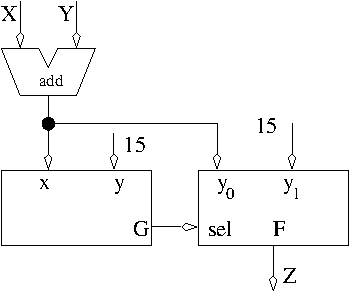
\includegraphics{./FigHw4/Sol4-10}

} \end{solution}

\item {\bf (10 pts.)} Build a mod-6 adder.  The mod-6 adder
takes as input two 3-bit (mod 6) numbers and adds them together
modulus 6.  

\index{modular arithmetic}
\label{page:mod}
Modular arithmetic only operates with a limited portion of the
integers.  The range of numbers is $\{0,1,2, \ldots ,m-1\}$ where 
$m$ is called the {\it modulus}; note there are $m$ different 
integers because counting started at 0.  For example, when working
in mod-6 arithmetic use the integers $\{0,1,2,3,4,5\}$.
To solve any addition problem in modular arithmetic, it is only 
necessary to perform regular addition with the special rule that 
the addition process rolls over from the largest number, $m-1$ to 0
when the result is larger than $m-1$.  For 
example, in mod-6 arithmetic $(5+1) \mod 6 = 0$.  The statement 
``$\mod 6$" is always included in the addition problem to indicate 
to the reader that mod-6 arithmetic is being performed.  Here
are a few more examples to help

\begin{tabular}{l}
$2+3~\mod 6 = 5$ \\
$3+3~\mod 6 = 0$ \\
$4+3~\mod 6 = 1$ \\
$5+5~\mod 6 = 4$ 
\end{tabular}

\index{modular adder}
\label{page:modadder}
\begin{tabular}{|l|p{3.5in}|} \hline
Nomenclature:  & 3-bit mod 6 adder                \\ \hline
Data Input:    & two, 3-bit (mod-6) vectors \verb+A, B+  \\ \hline
Data Output:   & 3-bit (mod-6) vector \verb+sum+    \\ \hline
Control:       & none                                   \\ \hline
Status:        & none                                   \\ \hline
Behavior:      & 
				\begin{verbatim}
				sum = A+B mod 6
				\end{verbatim}
		 \\ \hline
\end{tabular}

Submit a schematic showing the basic building blocks, their
data status, and control interconnections.  Show any truth
tables used to build glue logic.  Be careful that the word
size of the result is handled correctly.

\begin{solution}{
Since the inputs are mod 6 numbers then the inputs can be in the
range [0-5].  Adding two such values will yield a value in the 
range [0-10].  Hence a simple adjustment of the sum when its larger
that 5 is required.

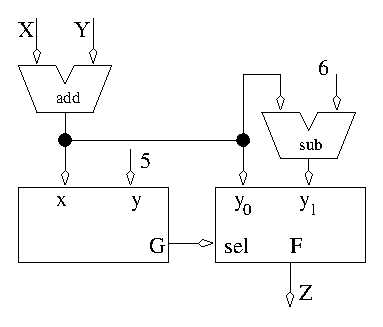
\includegraphics{./FigHw4/Sol4-11}

} \end{solution}

\item {\bf (1pt. each)}Convert the following to 2's-complement 
assuming a word size of eight bits. 
\begin{enumerate}
\item -35 

\begin{solution}{
$35 = 32+2+1 = 100011 = 00100011$, thus $-35=11011101$
} \end{solution}

\item  -128 

\begin{solution}{
This is a special case, see page 10 for more information.
$-128 = 10000000$
} \end{solution}

\item  67 

\begin{solution}{
$67=64+2+1 = 100 0011 = 0100 0011$
} \end{solution}

\item  128 

\begin{solution}{
There are not enough bits to represent this positive number; hence
the 8-bit representation does not exist.
} \end{solution}

\end{enumerate}


\item {\bf (1 pt. each)} Perform the following operations for the given 
2's-complement numbers. Assume a word size of eight bits
in all cases. Indicate where overflow occurs. If there is no overflow, 
convert the result to decimal. 
\begin{enumerate}

\item 01011101 + 00110111 

\begin{solution}{
 01011101 + 00110111 = 10010100  overflow
} \end{solution}

\item 11101011 + 11110001 

\begin{solution}{
 11101011 + 
 11110001 =
 11011100
} \end{solution}

\item 01011101 + 10101011 

\begin{solution}{
 01011101 + 
 10101011 =
 00001000
} \end{solution}

\item 10111011 - 11110001 

\begin{solution}{
 10111011 - 
 11110001 =

 10111011 +
 00001111 =
 11001010
} \end{solution}

\item 01011101 - 00110111 

\begin{solution}{
 01011101 - 
 00110111 =

 01011101 +
 11001001 =
 00100110
} \end{solution}

\item 01011101 - 10101111 

\begin{solution}{
 01011101 - 
 10101111 =

 01011101 +
 01010001 =
 10101110, overflow
} \end{solution}

\end{enumerate}

\item{\bf (5 pts.)} Build a 4-bit bus transceiver.  A bus transceiver
is defined by the following truth table.
                                                                                
\index{bus transceiver}
\label{page:bustranciever}
\begin{tabular}{|l|p{3.5in}|} \hline
Nomenclature:  & N-bit bus transceiver.                    \\ \hline
Data:          & two bidirectional N-bits vectors $X=x_{N-1} \ldots x_1 x_0$.                                                                                 
                        $Y=y_{N-1} \ldots y_1 y_0$.          \\ \hline
Control:       & 1-bit $F$ and $R$             \\ \hline
Status:        & none                                   \\ \hline
Behavior:      &
                        \begin{tabular}{c|c|c|c||c}
                        F  & R  & X & Y & comment \\ \hline
                        0  & 0  & Z & Z & X and Y tristate \\ \hline
                        0  & 1  & Y & Y & X = Y  \\ \hline
                        1  & 0  & X & X & Y = X  \\ \hline
                        1  & 1  & x & x & never applied \\
                        \end{tabular} \\ \hline
\end{tabular}
\label{page:bus}
\\ \\
Flow is determined by the $F$ and $R$ signals denoting forward and reverse
respectively.  When $F=1$, data flows from $X$ to $Y$.  In this case,
$X$ is acting like and input and $Y$ is acting like an output.  When
$R=1$, data flows from the $Y$ input to the $X$ output.  This design
relies heavily on tristate buffers.
                                                                                
\begin{solution} {
\begin{figure}[ht]
\center{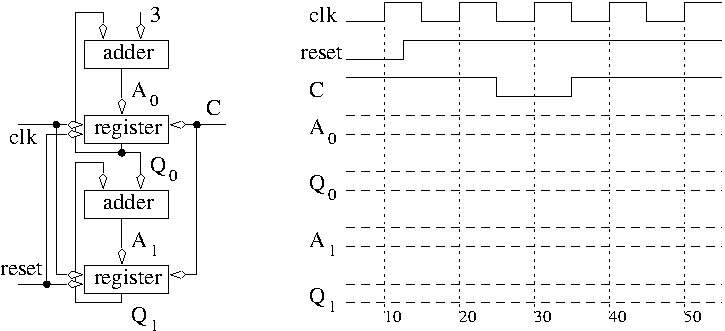
\includegraphics{./FigHw4/Prob4-16}}
\end{figure}
} \end{solution}
                                                                                
\item{\bf (3 pts.)} Build a 2:1 mux using some tristate buffers and an inverter.                                                                                
\item{\bf (3 pts.)} Build a 4:1 mux using some tristate buffers and two inverters.
                                                                                
\begin{solution} {
\begin{figure}[ht]
\center{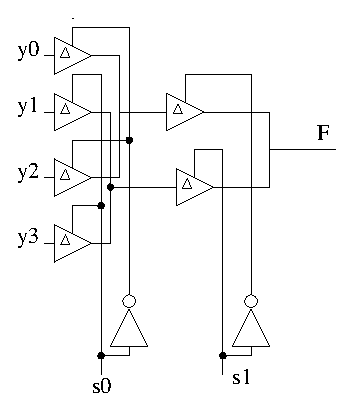
\includegraphics{./FigHw4/Prob4-17}}
\end{figure}
} \end{solution}
                                                                                
\item {\bf (10 pts.)}
\label{page:flipbox}
Build a flip box.  A flip box is defined by the following input,
output, and behavior definition.

\begin{tabular}{|l|p{3.5in}|} \hline
Nomenclature:  & 8-bit flip box.                    \\ \hline
Data Input:    & 8-bit $D=d_7 \ldots d_0$          \\ \hline
Data Output:   & 8-bit $F=f_7 \ldots f_0$          \\ \hline
Control:       & 3-bit $S=s_2 s_1 s_0$            \\ \hline
Status:        & none                                   \\ \hline
Behavior:      & The output is the same as the input except for
		one bit which is inverted.  The index of the inverted
		bit is given by $S$. \\ \hline
\end{tabular}

The flip box takes the 8-bit data input, flips a single bit identified
by $S$, then sends the new 8-bit value to the output.  
For example, if $D=11110000$ and $S=010$ then
$F=11110100$.  If $D=11110000$ and $S=101$ then $F=11010000$.  The solution
should rely heavily on the basic building blocks.

\begin{solution} {
Arrange 8, 2:1 muxes with $d_i$ and $d_i'$ going into the data inputs.
Run the select into a 3:8 decoder and route the data outputs to the 
individual selects of the 2:1 muxes.
} \end{solution}


\item {\bf (10 pts.)}
\label{page:IsScan}
Build a box which recognizes some keyboard scancode.  When a key is 
pressed on a keyboard, the keyboard transmits (among other things) 
an 8-bit scancode of the pressed key.  Each key has its own scancode 
listed in Table~\ref{table:scancodes}.  The relationship between the 
keys and their scancode is not based on ASCII.

\begin{table}
\begin{tabular}{|l|l||l|l||l|l||l|l|} \hline
Key & scancode & Key & scancode & Key & scancode & Key & scancode \\ \hline \hline 
0 & $45_{16}$ & 1 & $16_{16}$ & 2 & $1E_{16}$ & 3 & $26_{16}$ \\ \hline
4 & $25_{16}$ & 5 & $2E_{16}$ & 6 & $36_{16}$ & 7 & $3D_{16}$ \\ \hline
8 & $3E_{16}$ & 9 & $46_{16}$ & A & $1C_{16}$ & B & $32_{16}$ \\ \hline
C & $21_{16}$ & D & $23_{16}$ & E & $24_{16}$ & F & $2B_{16}$ \\ \hline
P & $4D_{16}$ & L & $4B_{16}$ & M & $3A_{16}$ & I & $43_{16}$ \\ \hline
\end{tabular}
\caption{Some keyboard scancodes.}
\label{table:scancodes}
\end{table}

\label{page:scanclass}
\begin{tabular}{|l|p{3.5in}|} \hline
Nomenclature:  & scancode classifier                   \\ \hline
Data Input:    & 8-bit $D=d_7 \ldots d_0$          \\ \hline
Data Output:   & IsP, IsL, IsM, IsI, IsS \\ \hline
Control:       & none             \\ \hline
Status:        & none                                   \\ \hline
Behavior:      & IsP =1 when $D$ is the scan code for the letter ``P".
		 IsL =1 when $D$ is the scan code for the letter ``L".
		 IsM =1 when $D$ is the scan code for the letter ``M".
		 IsI =1 when $D$ is the scan code for the letter ``I".
		 IsS =1 when $D$ is the scan code for the letter ``S".  \\ \hline
\end{tabular}

\item {\bf (10 pts.)}
\label{page:ScanDecode}
Build a box which converts an 8-bit scancode for a hexadecimal
digit into a 4-bit hexadecimal values.

\label{page:scanconv}
\begin{tabular}{|l|p{3.5in}|} \hline
Nomenclature:  & scancode classifier                   \\ \hline
Data Input:    & 8-bit $D=d_7 \ldots d_0$          \\ \hline
Data Output:   & 4-bit $H=h_3h_2h_1h_0$ \\ \hline
Control:       & none             \\ \hline
Status:        & none                                   \\ \hline
Behavior:      & Converts the scancode $D$, representing a the
		key of a hexadecimal character, into its 4-bit 
		value $H$.
		 \\ \hline
\end{tabular}

For example, if $D=25_{16}$, the scancode for the "4" key, then the converter
should output $H=0100_2$.  Assume that the inputs are always
legal hexadecimal scancodes.

\end{enumerate}


\end{document} 
